\mysubsection{Commande Angulaire et Cartésienne}

\subsubsection{Commande Angulaire}

Pour la commande dans l'espace des articulations, on a mis en \oe{}uvre sur Matlab et Simulink les techniques de commande montrées dans le subsection \ref{Comm_Ang}. On a évalué les peformances de chaque méthode en tenant compte de la réponse à une consigne de position angulaire en échellon filtrée par un système de premier ordre et constante de temps de 0.5s, ainsi que des efforts de commande nécessaires. 

On a choisi comme pulsation de brisure $ \omega$ = $ 10$ $rad/s $ pour toutes les articulations, pour des critères de comparaison. Il est possible de augmenter la fréquence de brisure afin de réduire le temps de réponse du système, mais comme il a été dit, cela peut apporté des efforts de commande trop importants. La choix définitive de cette pulsation doit être fait après l'integration de la commande avec le robot.
\\

\textbf{Commande angulaire PID}
\\

Les résultats obtenus pour la commande angulaire PID, avec une consigne de $ \left[0, 0, -\frac{\pi}{2}, 0, \frac{\pi}{2} \right] $ en ce qui concerne l'évolution temporelle des positions angulaire et des efforts de commande sur chaque articulation sont montrés dans la suite.

\begin{figure}[H]
	\begin{center}	
		\captionsetup{justification=centering,margin=1cm}
		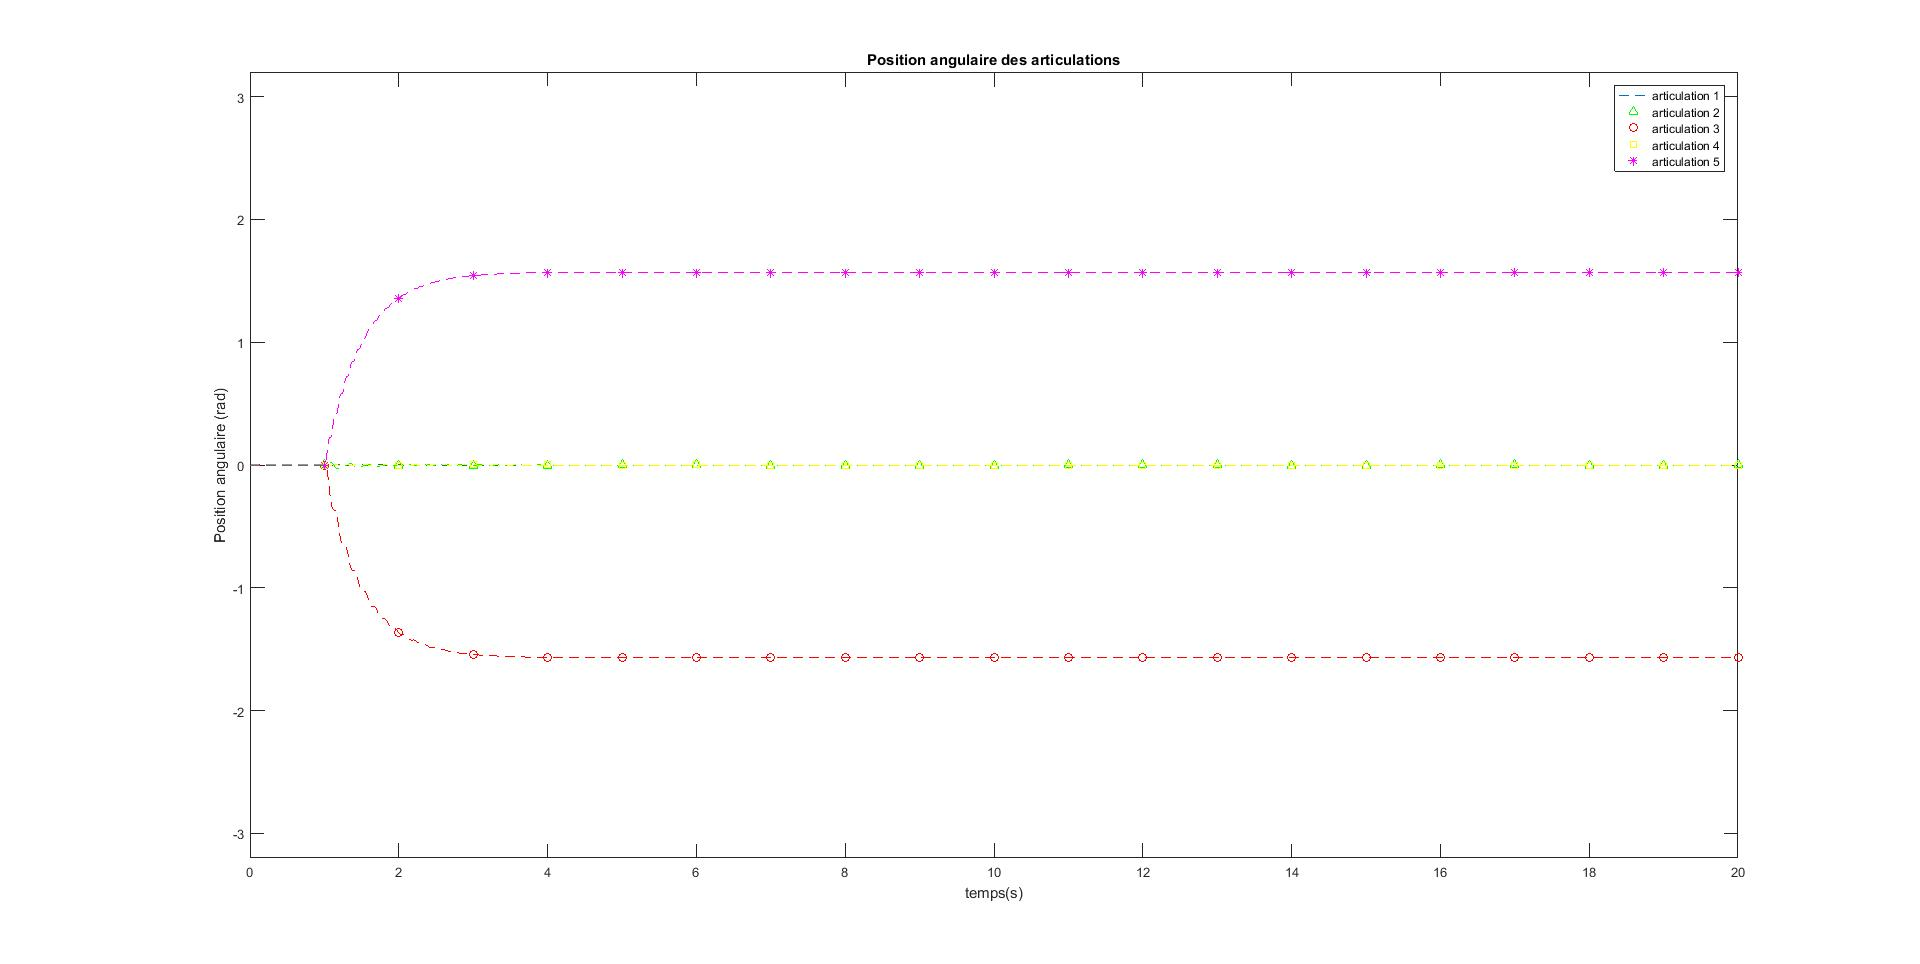
\includegraphics[width=\textwidth]{./res_position_PIDjoint.JPG}
		\caption{Réponse temporelle du système commandé par un PID dans l'espace articulaire}
		\label{fig:PID_joint_space_response}
	\end{center}
\end{figure}

\begin{figure}[H]
	\begin{center}
		\captionsetup{justification=centering,margin=1cm}	
		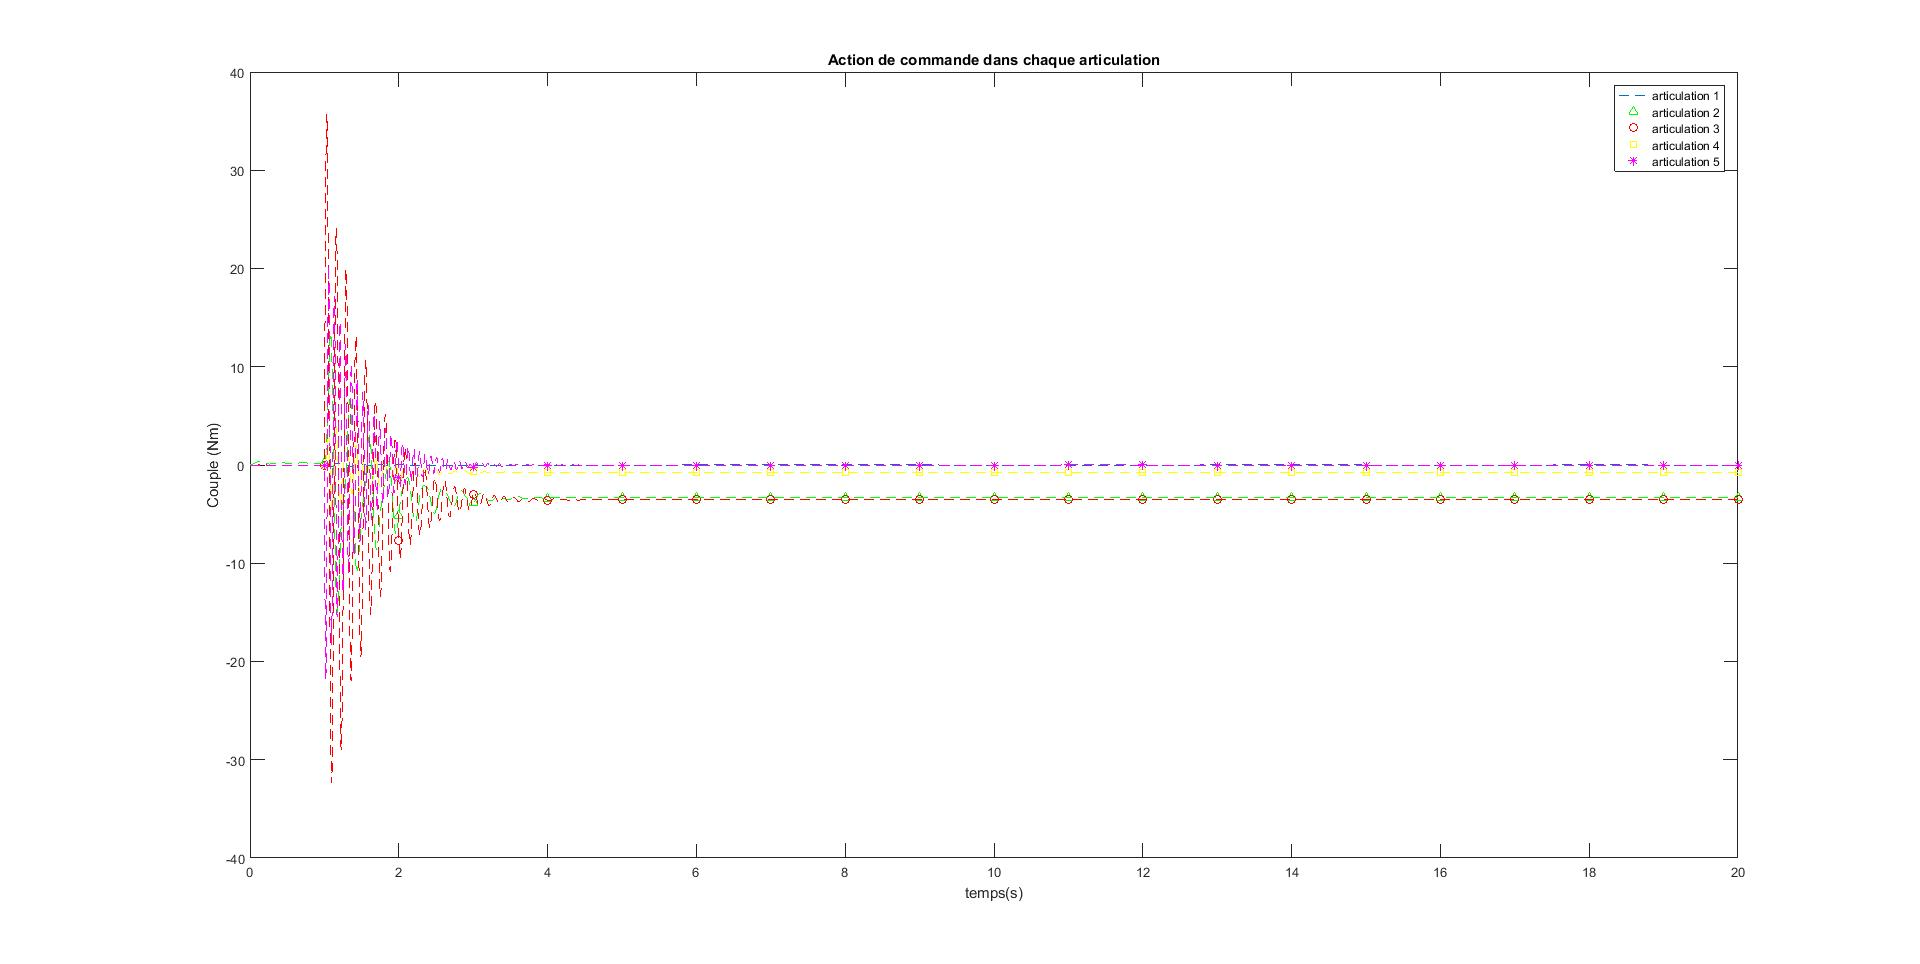
\includegraphics[width=\textwidth]{./res_commande_PIDjoint.JPG}
		\caption{Efforts de commande appliqués au système commandé par un PID dans l'espace articulaire }
		\label{fig:PIDjointcontgraph}
	\end{center}
\end{figure}

On peut noter dans les graphiques que le robot atteint bien la position voulue avec des efforts de commande en régime qui sont non nuls pour compenser l'action de la gravité, mais qui ne sont pas aussi trop importants. Il existe des petites fluctuations dans la réponse transitoire de la position angulaire, mais elles ne gênent pas beaucoup la dynamique du système. Le seul problème est que l'effort de commande devient plus important au début pour démarrer le mouvement du robot.

On a refait les graphiques en supposant que les mesures de position sont bruités. Le bruit considéré est un bruit blanc avec une variance de $ 10^(-4) $. On n'a pas trouvé d'information à propos des capteurs du robot, mais il serait mieux si on avait choisi cette variance pour être équivalent à la précision de ce capteur.

\begin{figure}[H]
	\begin{center}	
		\captionsetup{justification=centering,margin=1cm}
		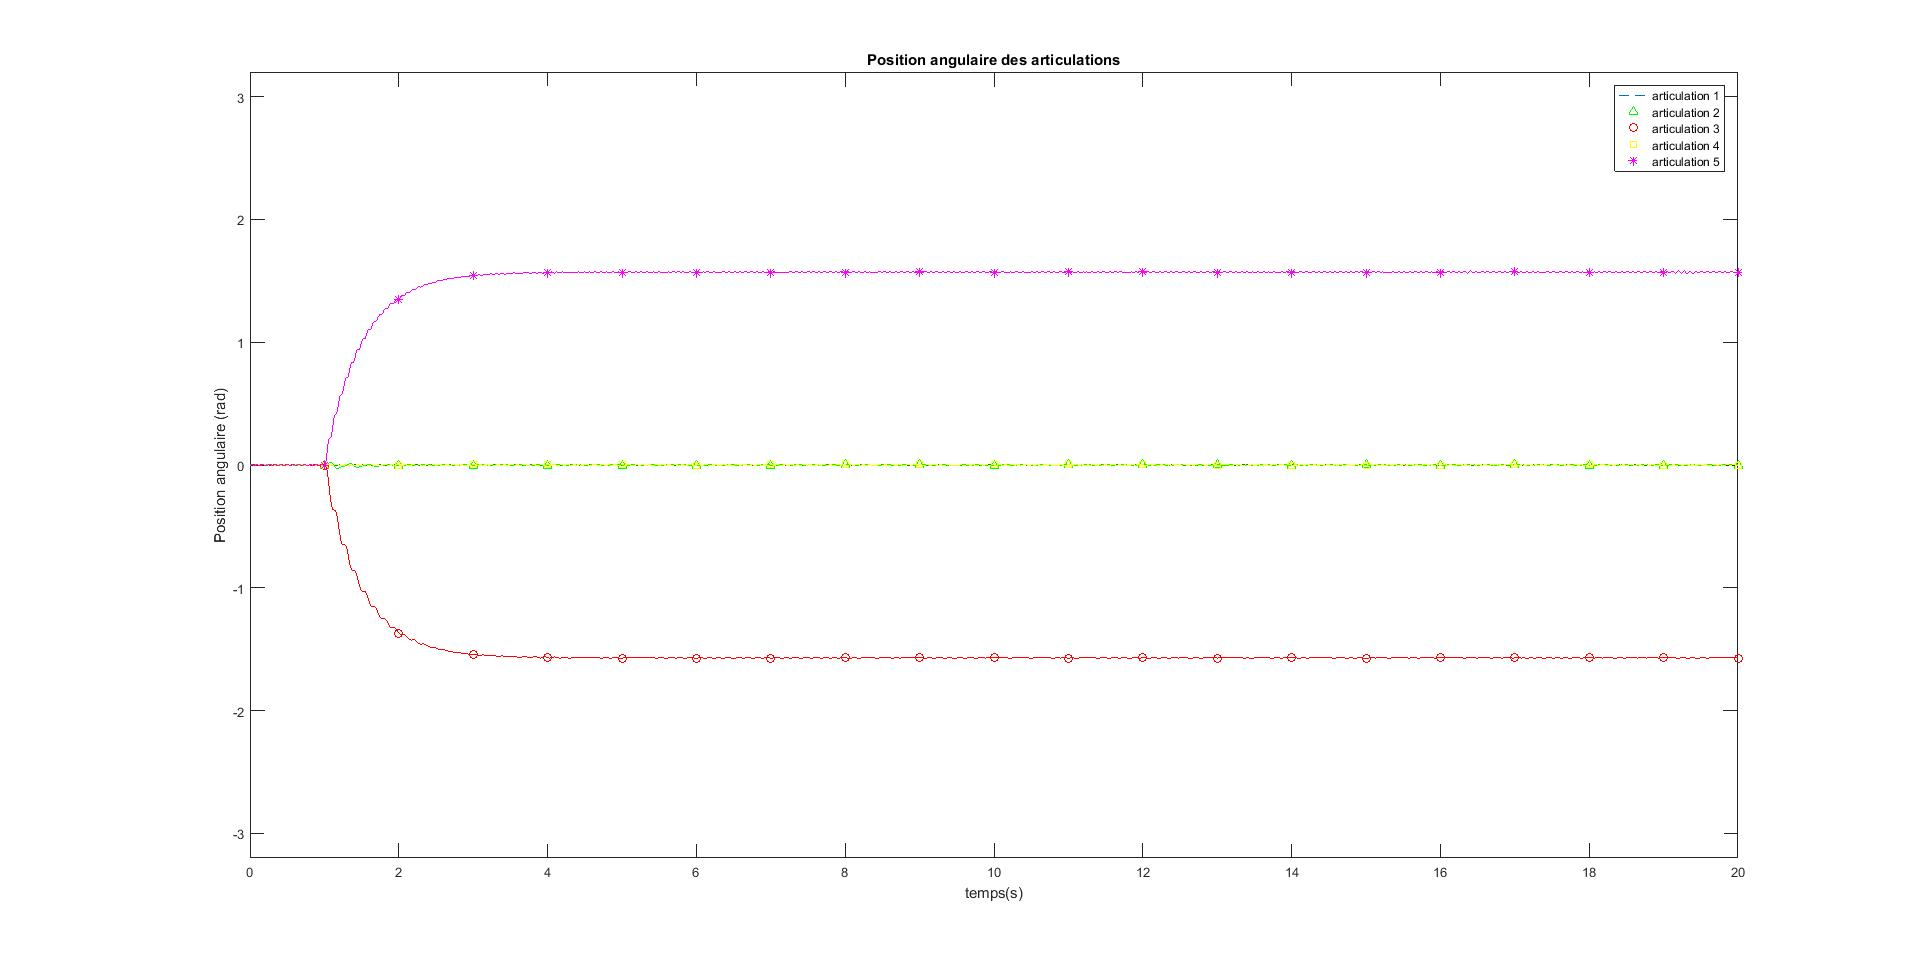
\includegraphics[width=\textwidth]{./res_position_PIDjoint_dist.JPG}
		\caption{Réponse temporelle du système commandé par un PID dans l'espace articulaire avec perturbation de mesure}
		\label{fig:PID_joint_space_response_dist}
	\end{center}
\end{figure}

\begin{figure}[H]
	\begin{center}
		\captionsetup{justification=centering,margin=1cm}	
		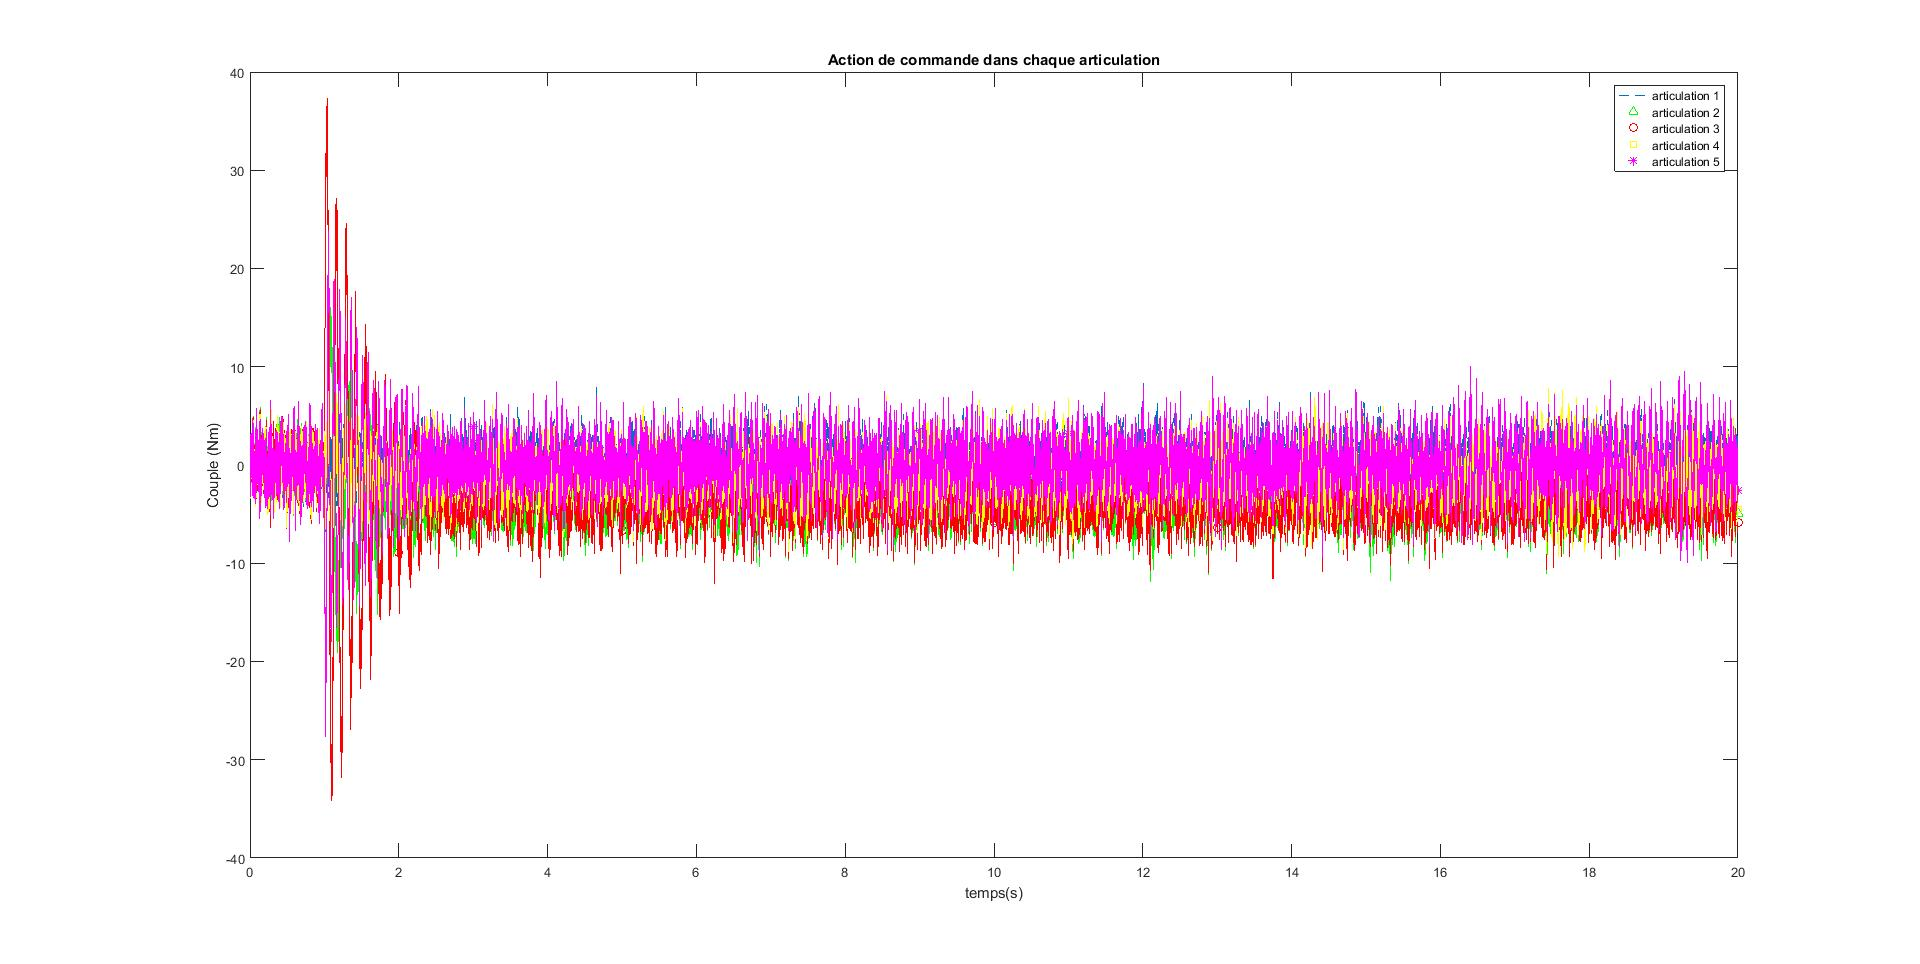
\includegraphics[width=\textwidth]{./res_commande_PIDjoint_dist.JPG}
		\caption{Efforts de commande appliqués au système commandé par un PID dans l'espace articulaire avec perturbation de mesure}
		\label{fig:PIDjointcontgraphdist}
	\end{center}
\end{figure}

Malgré le petit bruit présent au régime, la réponse de la position angulaire reste stable. Par contre, les efforts de commande deviennet très bruit pour maintenir cette stabilité de position, en dépit de ne pas atteindre des valeurs beaucoup plus élevées que dans le cas précédent. De toute façon, il y a des soucis pour la commande PID si la précision des capteurs est faible. 
\newline

\textbf{Commande angulaire par couple calculé}
\newline

Pour la commande angulaire par couple calculé, on a généré les mêmes graphiques en simulation que pour la commande PID, avec la même consigne de $ \left[0, 0, -\frac{\pi}{2}, 0, \frac{\pi}{2} \right] $. Les résultats sont montrés dans la suite.

\begin{figure}[H]
	\begin{center}
		\captionsetup{justification=centering,margin=1cm}	
		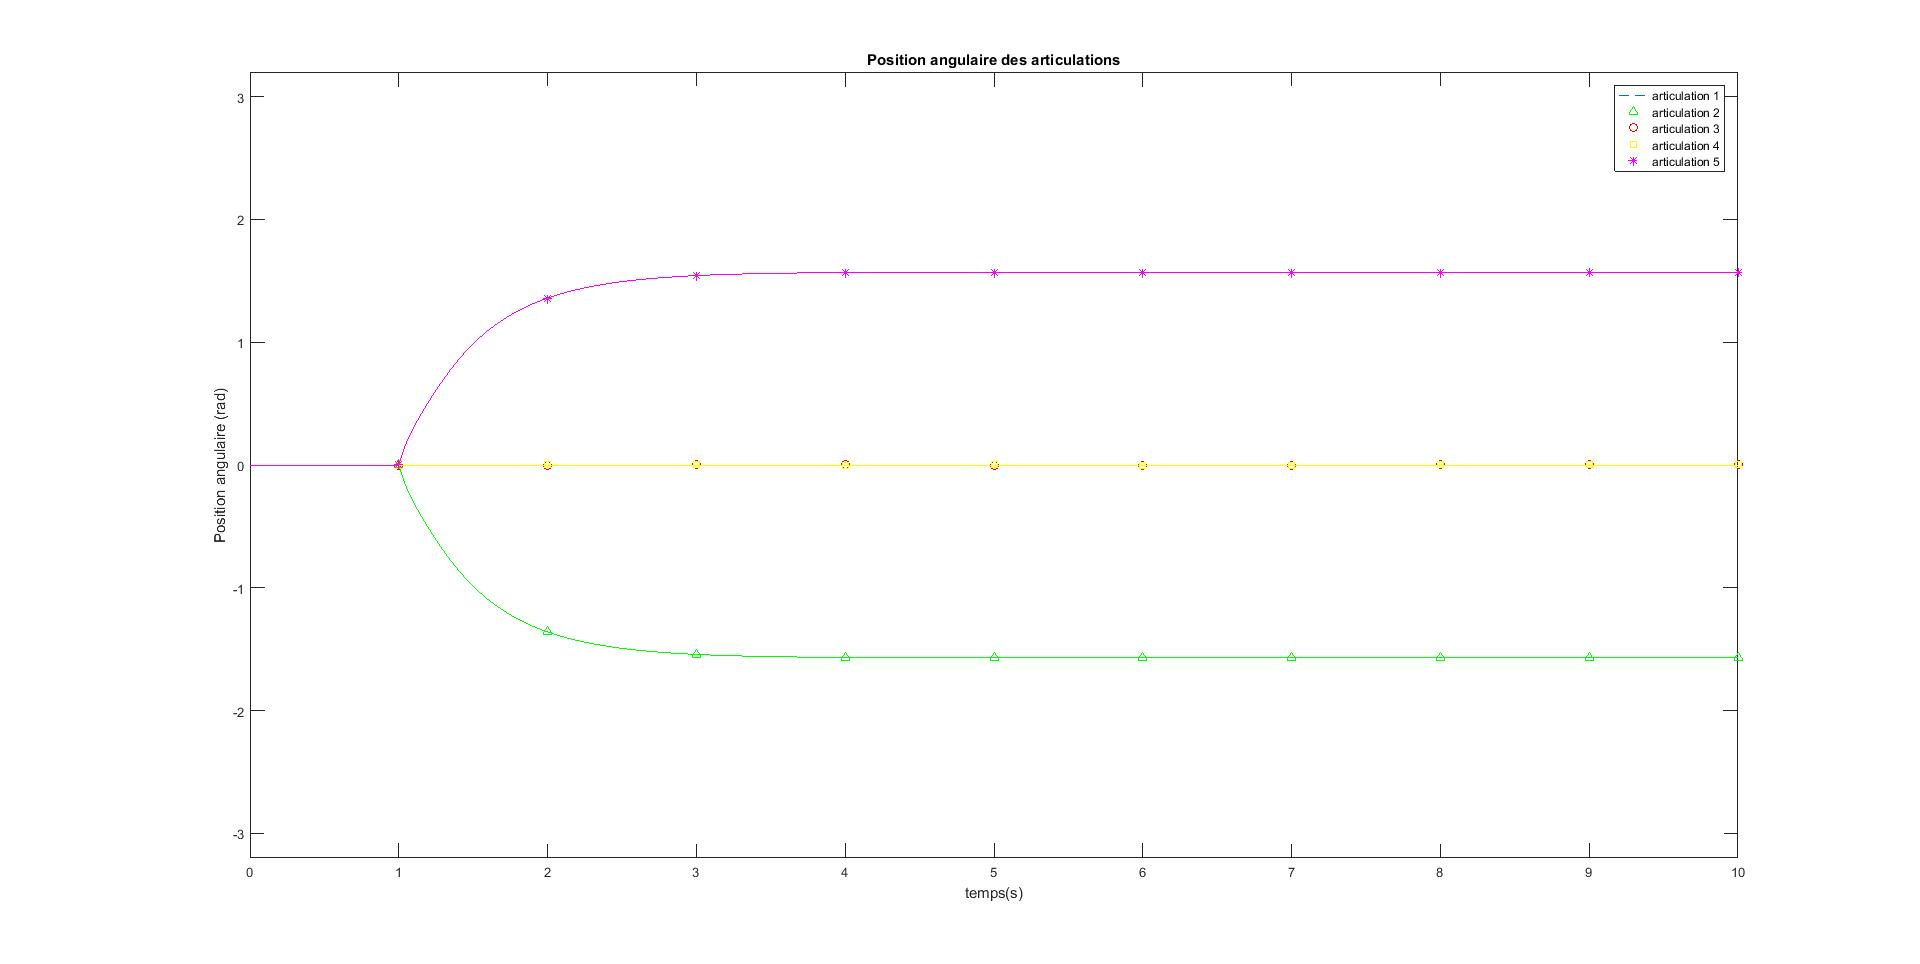
\includegraphics[width=\textwidth]{./res_position_CTIjoint.JPG}
		\caption{Réponse temporelle du système commandé par la méthode du couple calculé dans l'espace articulaire}
		\label{fig:CTI_joint_space_response}
	\end{center}
\end{figure}

\begin{figure}[H]
	\begin{center}	
		\captionsetup{justification=centering,margin=1cm}
		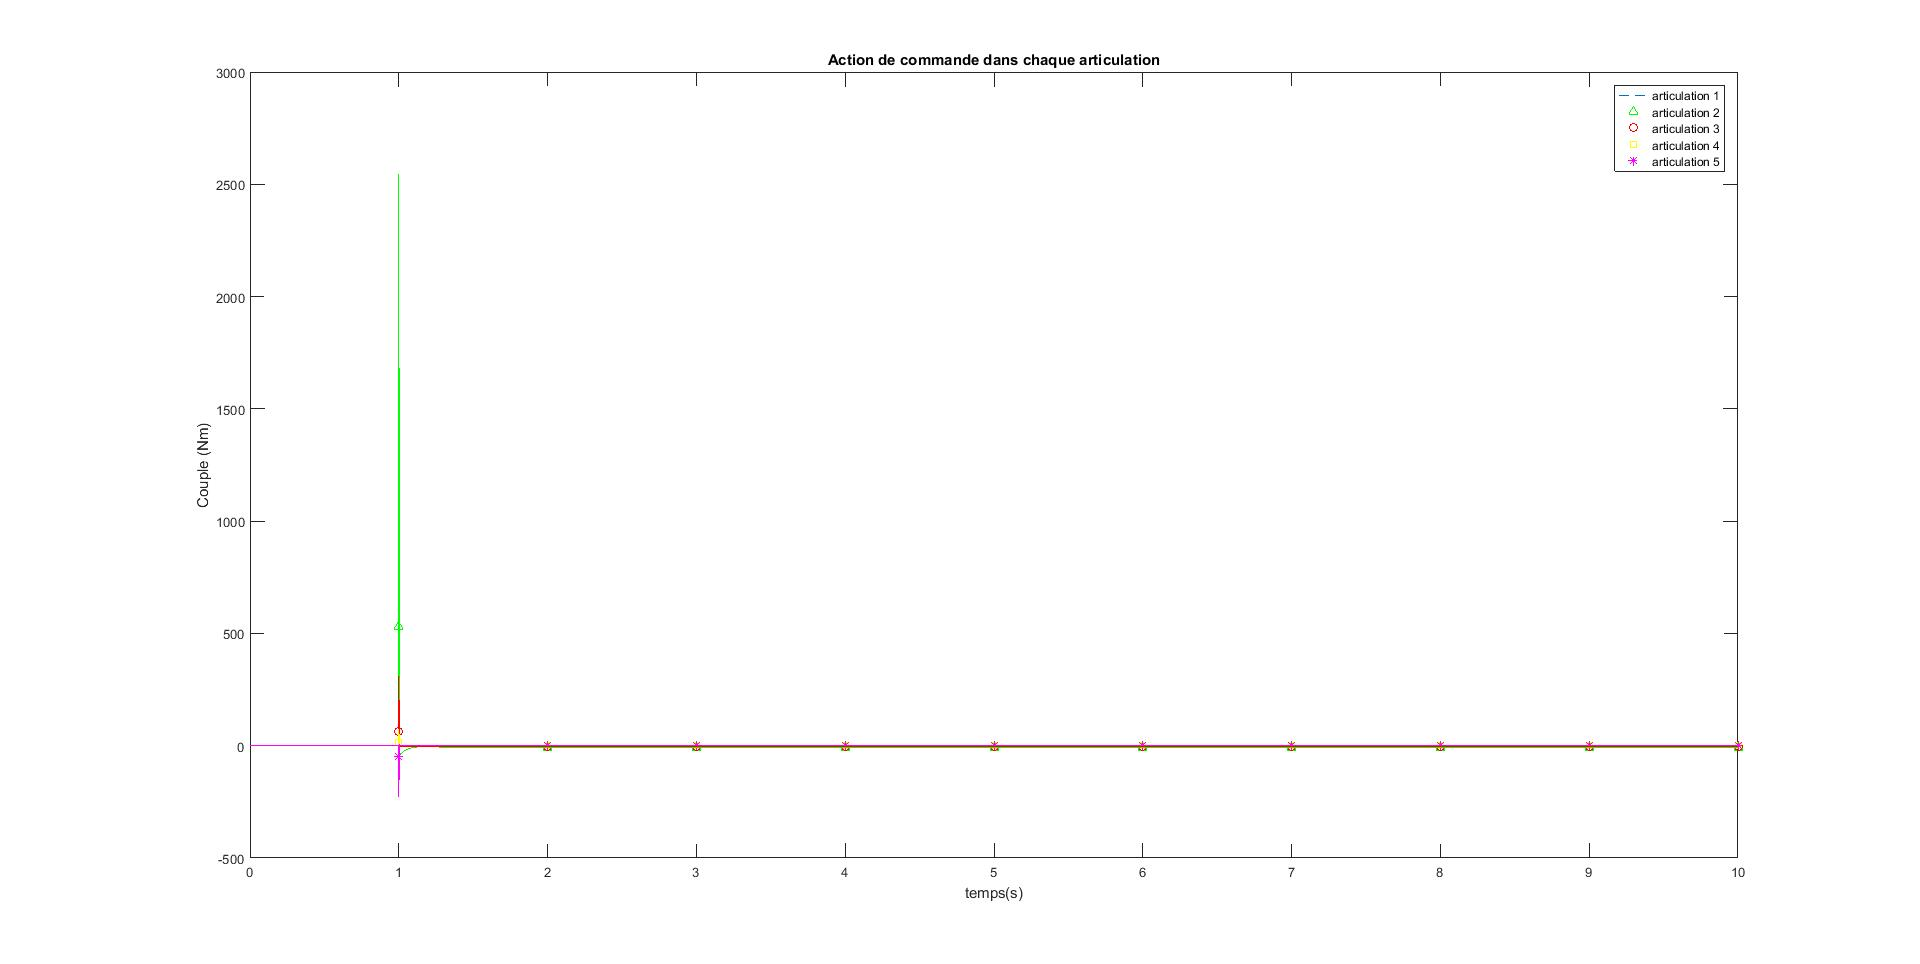
\includegraphics[width=\textwidth]{./res_commande_CTIjoint.JPG}
		\caption{Efforts de commande appliqués au système commandé par par la méthode du couple calculé dans l'espace articulaire}
		\label{fig:CTIgraphcont}
	\end{center}
\end{figure}

On peut noter dans ces graphiques qu'on a réduit les fluctuations de la réponse, une fois qu'on considère que le modèle est bien adapté au système et de cette façon, on compense les non-linérités. Par contre, cette avantage vient avec le coûte d'augmenter considérablement les efforts de commande dans le transitoire de la réponse.

Ensuite, on a essayé aussi de simuler des problèmes qu'on peut avoir lorsque la commande est intégrer au robot: on a ajouté un bruit blanc avec une variance de $ 10^(-2) $ dans la mesure des positions angulaires, on a determiné la vitesse angulaire par dérivation numérique de la position et on a ajouté une desadaptation de 5\% dans quelques paramètres du modèle par rapport au système. Les résultats sont montrés dans les graphiques suivants.

\begin{figure}[H]
	\begin{center}	
		\captionsetup{justification=centering,margin=1cm}
		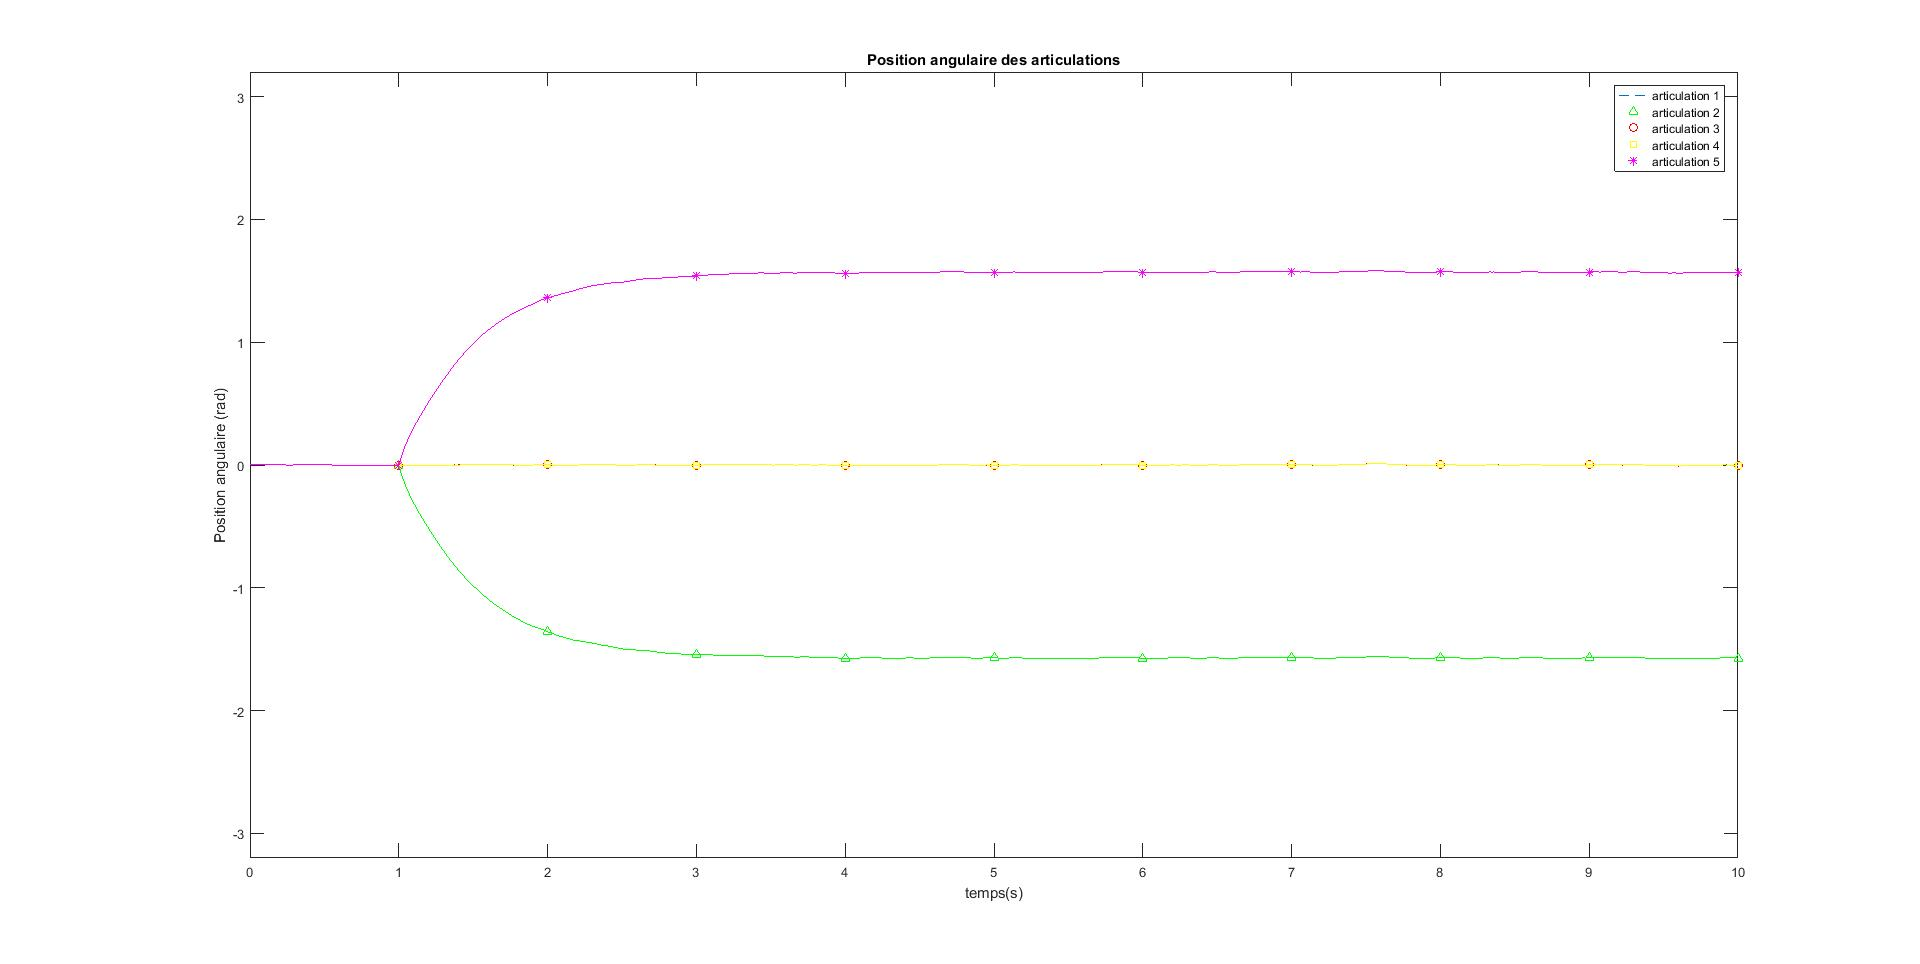
\includegraphics[width=0.95\textwidth]{./res_position_CTIjoint_dist.JPG}
		\caption{Réponse temporelle du système commandé par la méthode du couple calculé dans l'espace articulaire avec perturbation de mesure et desadaptation du modèle}
		\label{fig:CTIdistpos}
	\end{center}
\end{figure}

\begin{figure}[H]
	\begin{center}	
		\captionsetup{justification=centering,margin=1cm}
		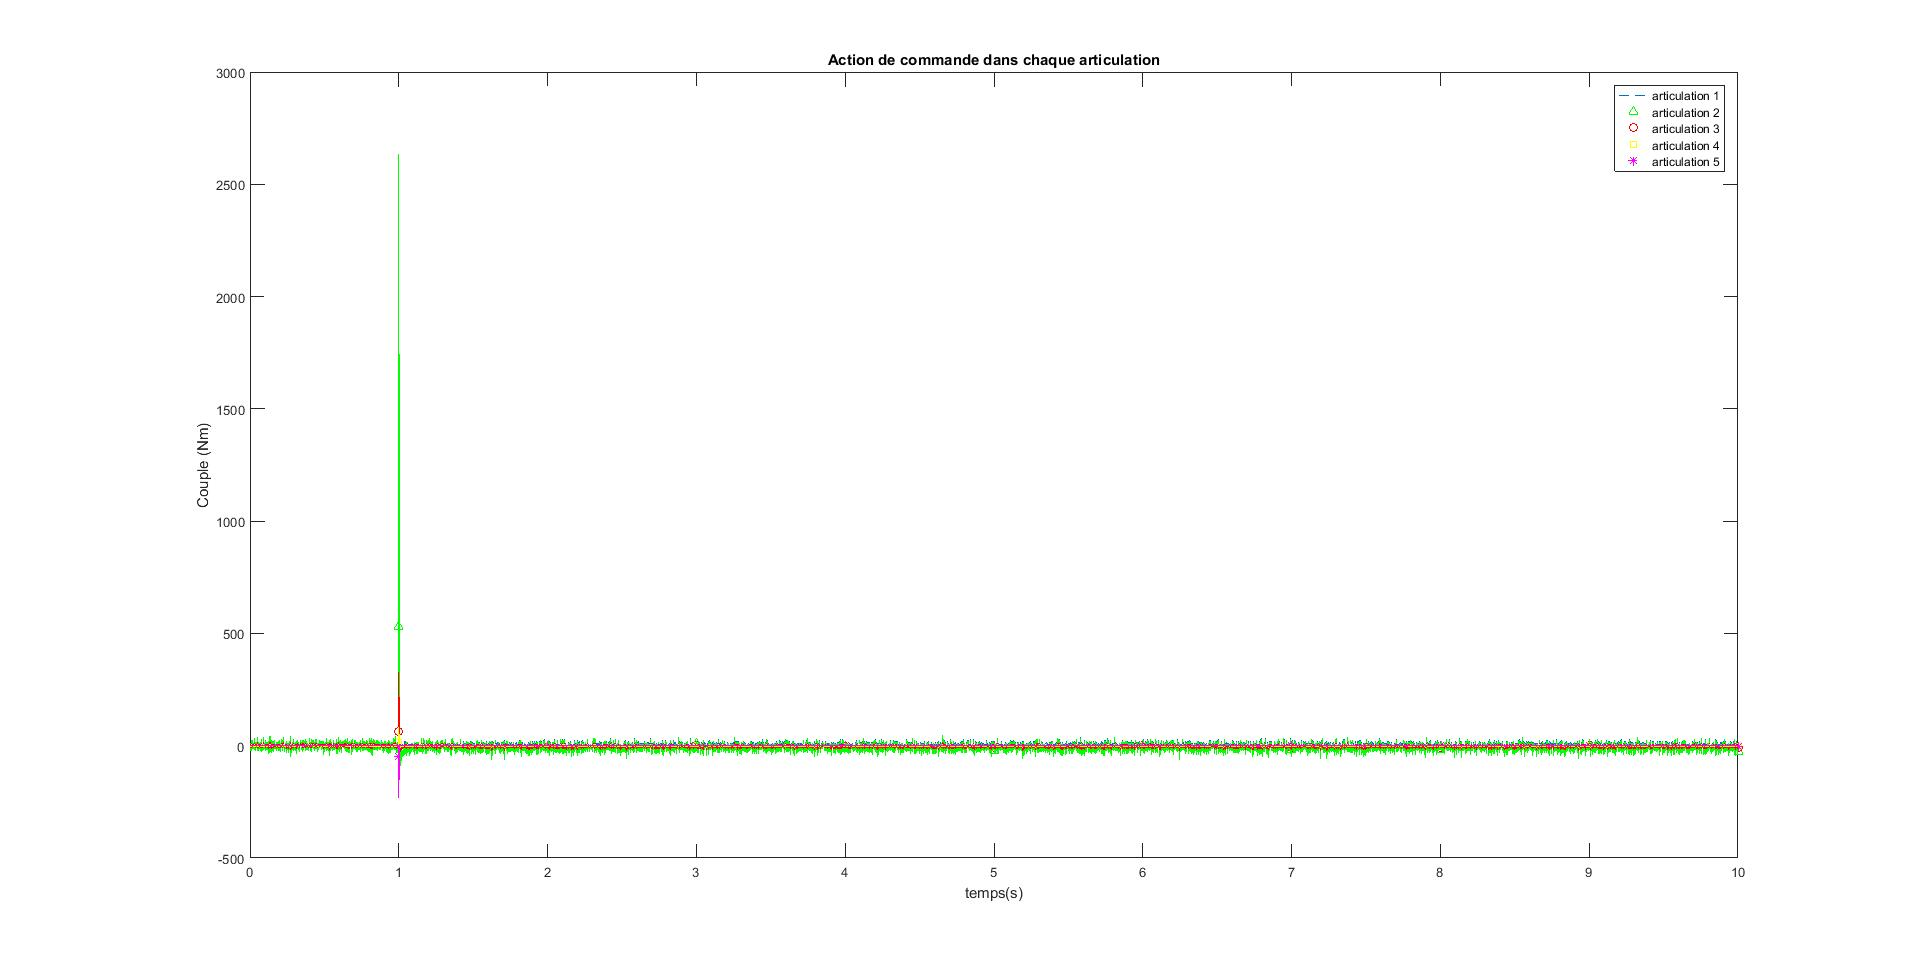
\includegraphics[width=0.95\textwidth]{./res_commande_CTIjoint_dist.JPG}
		\caption{Efforts de commande appliqués au système commandé par par la méthode du couple calculé dans l'espace articulaire avec perturbation de mesure et desadaptation du modèle}
		\label{fig:CTIdistcont}
	\end{center}
\end{figure}

Cette méthode de commande est moins sensible aux bruits de mesure que la dernière, parce qu'on a jouter une bruit avec une variance plus importante et le signal de sortie est moins bruité. Par contre, les efforts de commande sont aussi bruité que pour la commande PID.

Une prochaine étape pour cette projet serait ajouter les limitations angulaires, de vitesse et de couples des moteurs des articulation dans le modèle Simulink pour analyser les performances de la commande dans un cas un peu plus réel avant de l'intégrer au robot. On n'a pas ajouter ses limitations parce que on a trouver dans le mauel du fabriquant juste les limitations angulaires. Il faudra faire une recherche plus detaillé, ou même contacté les fabriquants pour obtenir ces informations.
\newpage
\subsubsection{Commande Cartésienne}

Pour la commande dans l'espace opérationnel, on a mis en \oe{}uvre sur Matlab et Simulink les techniques de commande montrées dans le subsection \ref{Comm_Cart}. En plus de tenir en compte la réponse temporelle des positions angulaires et de la position de l'outil à des consignes en échellon filtré et les efforts de commande pour évaluer les peformances de chaque méthode, on a considérer aussi la capacité du systè commandé de suivre des trajectoires linéaires ou circulaires.  
\newline

\textbf{Commande cascade avec boucle interne de vitesse angulaire}
\newline

La commande cascade avec boucle interne de vitesse angulaire a été mis en \oe{}uvre sur Matlab Simulink pour commander la position de l'outil du robot. Par contre, on n'a pas eu le temps d'adapter cette méthode pour commander aussi l'orientation de l'outil, parce qu'on nas pas réussi encore de calculer les vitesses de rotation du repère associé à l'outil par rapport au repère associé à la base du robot. On a toute la trajectoire de réference pour le robot décrite par des matrices hmogènes, il manque juste de les utiliser pour calculer les vitesses de rotation.

Dans la suite, on a les graphiques de la position de l'outil par rapport à la base du robot, des position angulaires et des efforts apliqués à chaque articulation pour une trajectoire linéaire et pour une trajectoire circulaire.

On observe que, pour les deux types de trajecoires, le robot les suit très bien, presque sans aucun erreur. Les mouvements angulaires réalisés sont lisses et se stabilisent aprés la fin de la trajectoire. Les efforts de commande restent avec des valeurs peu importants malgré quelque bruit existant. Ce bruit est du á la déterminaion de la consigne de vitesse angulaire pour le robot, qui est faite de façon numérique avec un bloc "dérivé" du Simulink. Il existe autres maniéres numérique de faire cette estimation, que conduisent à des résultats plus fiables et moins bruités, mais on n'a pas eu le temps de les mettre en \oe{}vre.

\begin{figure}[H]
	\begin{center}	
		\captionsetup{justification=centering,margin=1cm}
		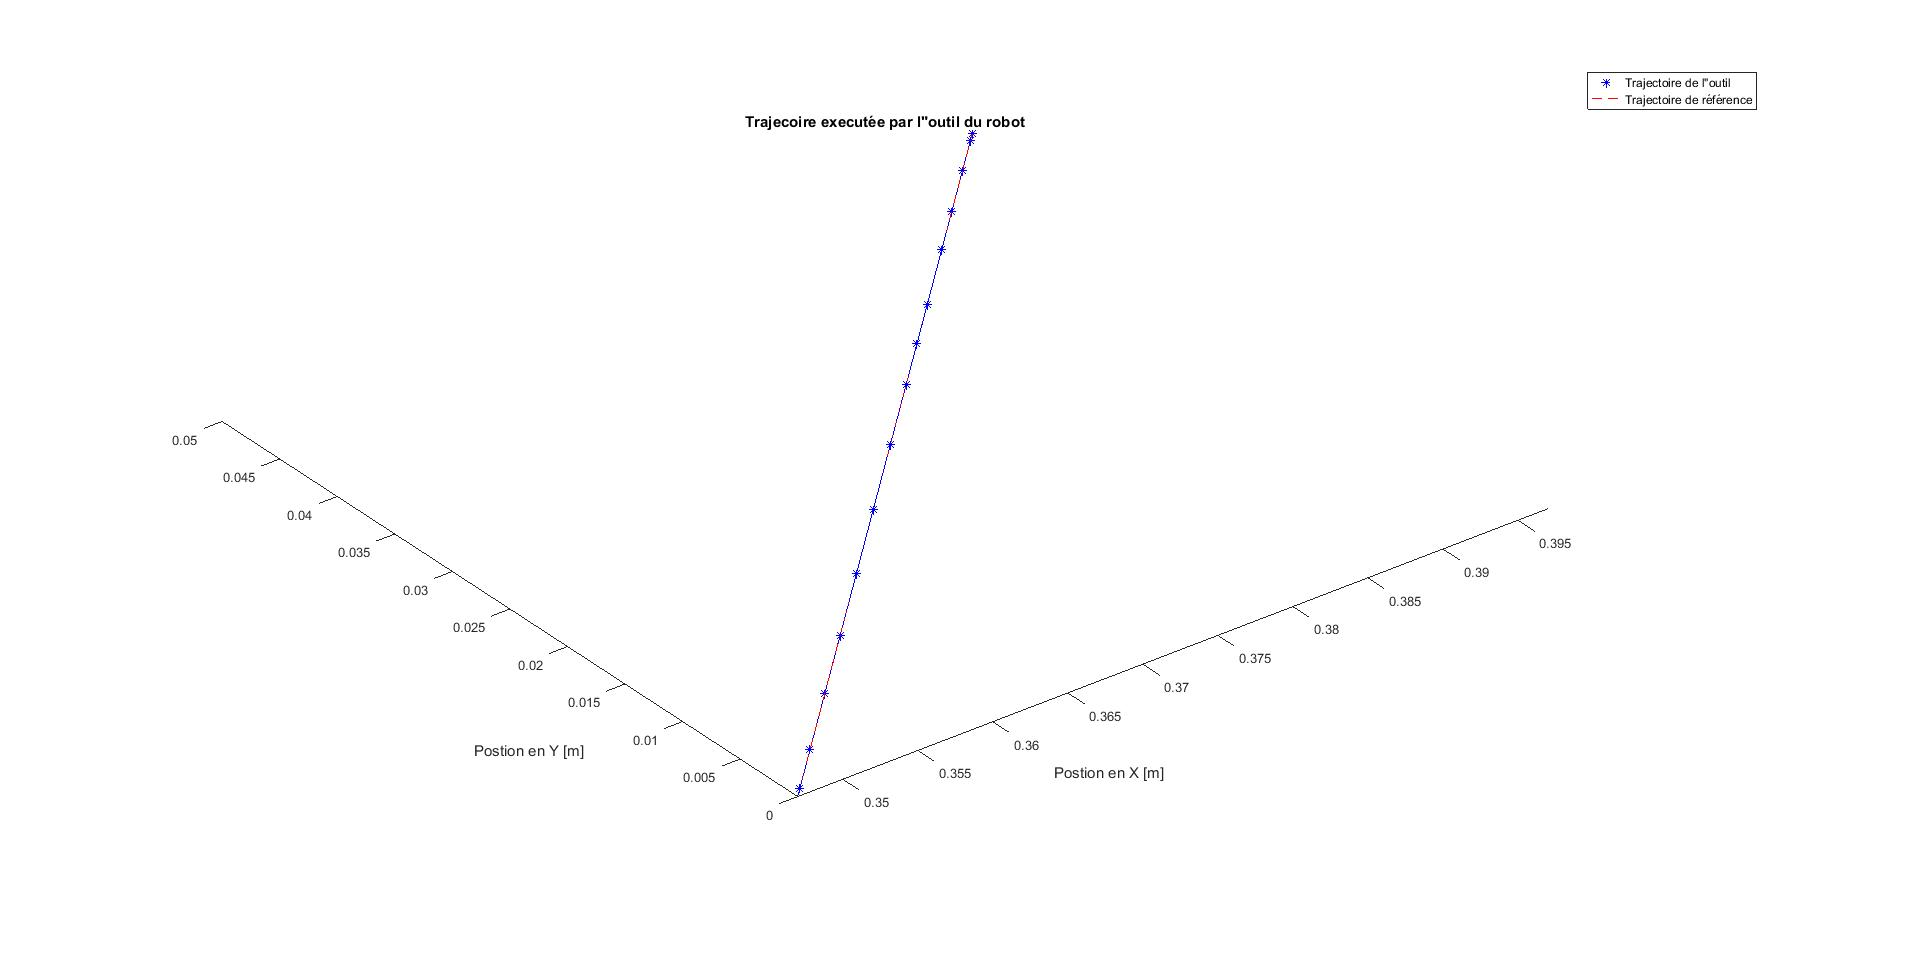
\includegraphics[width=\textwidth]{./Ltraj_positionLin_cascade.JPG}
		\caption{Comparaison de la trajectoire éxécutée par l'outil du robot commandé par la méthode cascade et la trajectoire de référence linéaire}
		\label{fig:Ltraj_positionLin_cascade}
	\end{center}
\end{figure}

\begin{figure}[H]
	\begin{center}
		\captionsetup{justification=centering,margin=1cm}	
		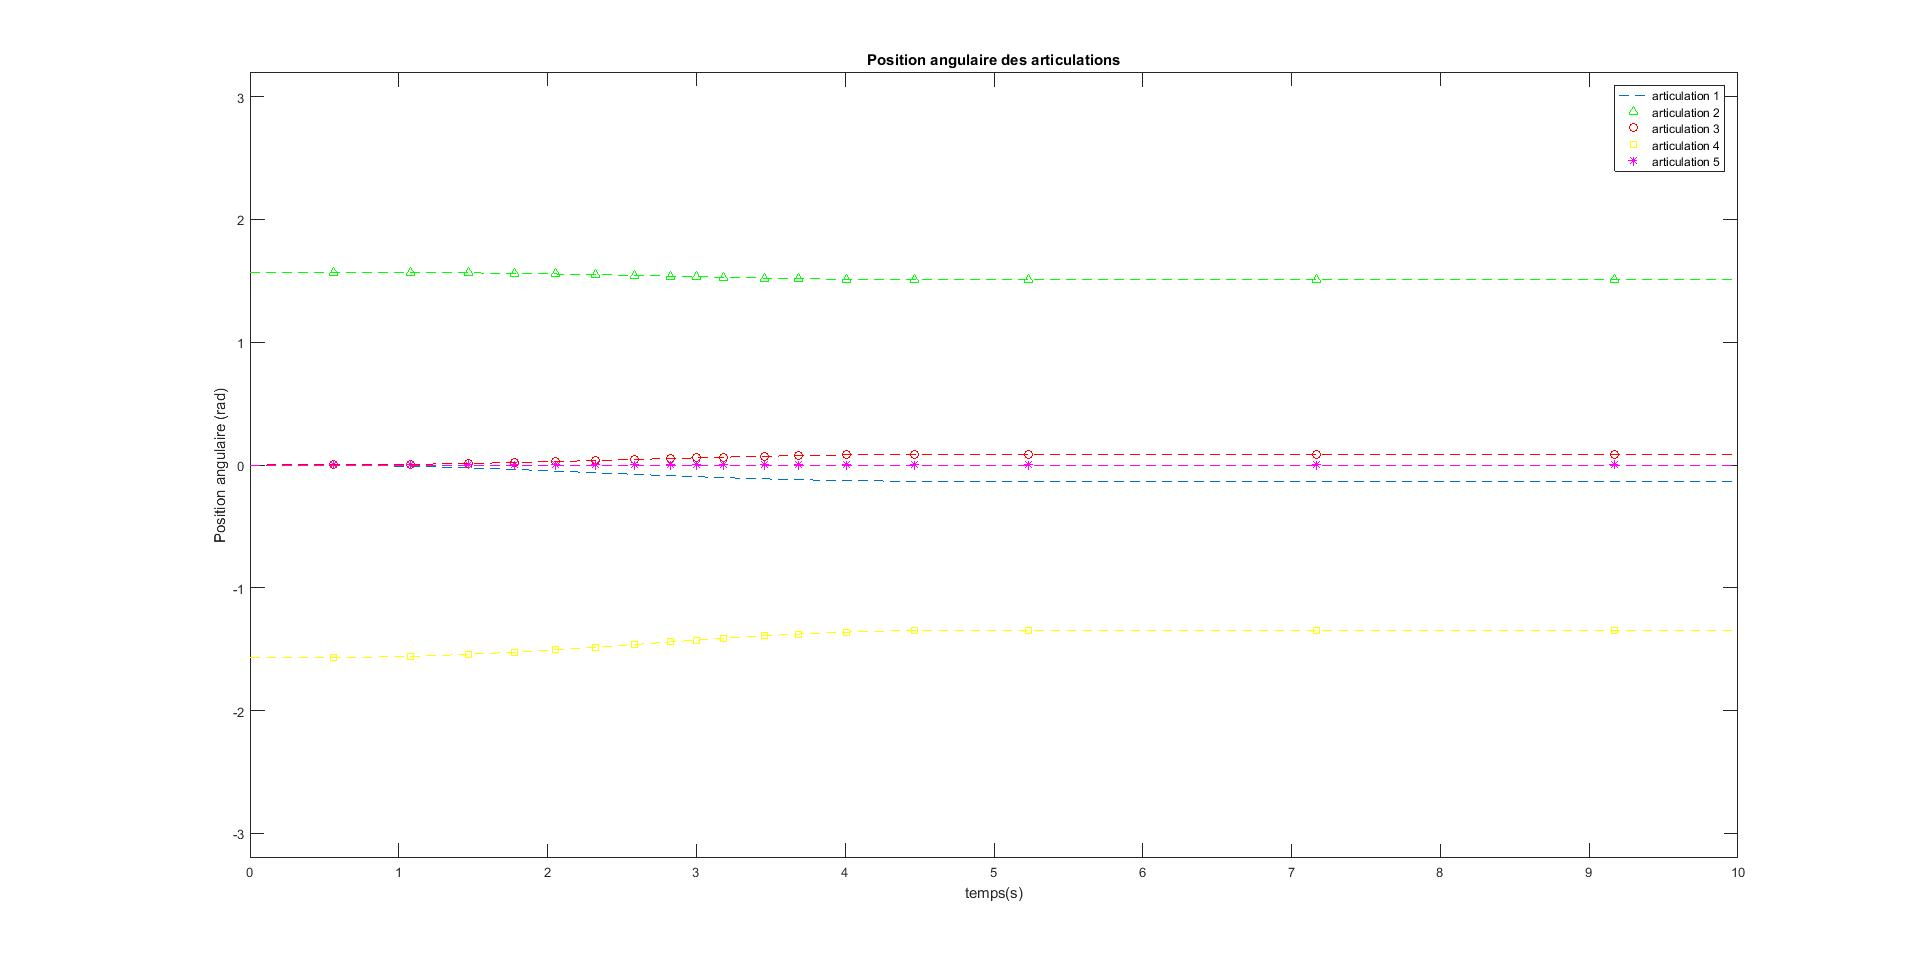
\includegraphics[width=\textwidth]{./Ltraj_positionAng_cascade.JPG}
		\caption{Réponse temporelle des positions angulaires des axes du robot commandé par la méthode cascade pour suivre une trajectoire linéaire}
		\label{fig:Ltraj_positionAng_cascade}
	\end{center}
\end{figure}

\begin{figure}[H]
	\begin{center}
		\captionsetup{justification=centering,margin=1cm}	
		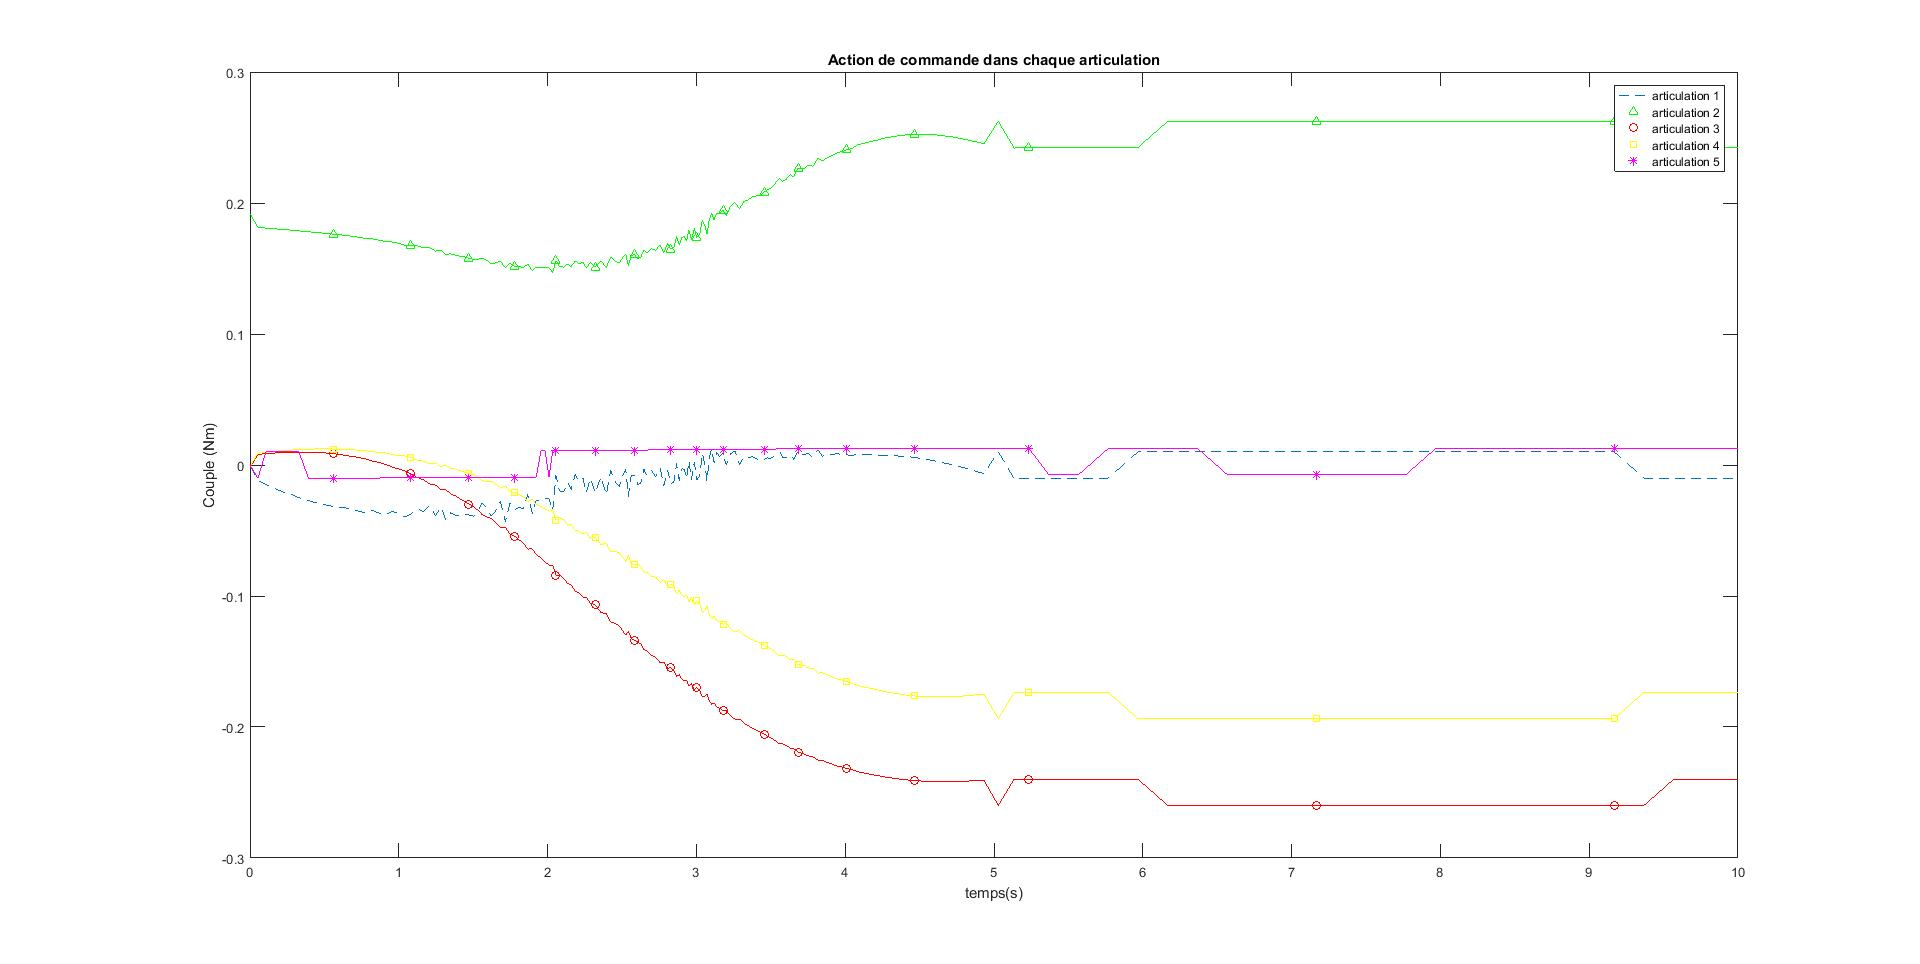
\includegraphics[width=\textwidth]{./Ltraj_commande_cascade.JPG}
		\caption{Efforts de commande appliqués aux articulations du robot commandé par la méthode cascade pour suivre une trajectoire linéaire}
		\label{fig:Ltraj_commande_cascade}
	\end{center}
\end{figure}
\newpage
\begin{figure}[H]
	\begin{center}	
		\captionsetup{justification=centering,margin=1cm}
		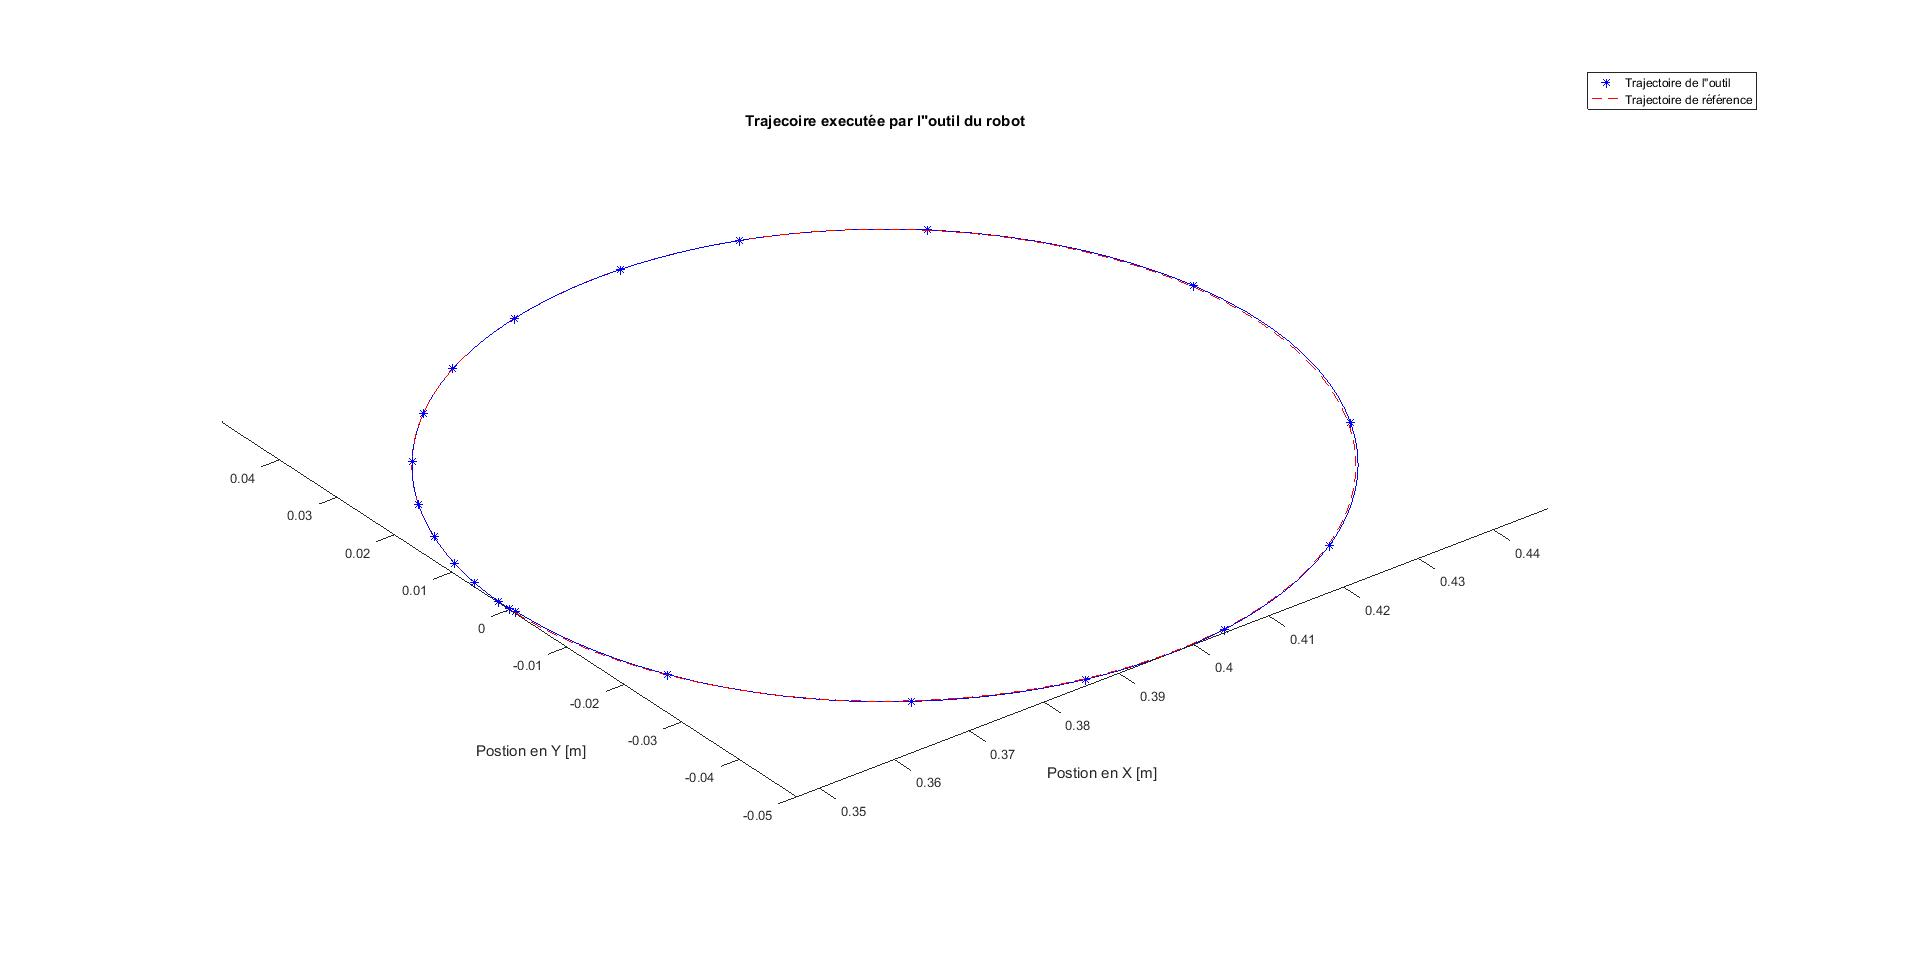
\includegraphics[width=\textwidth]{./Ctraj_positionLin_cascade.JPG}
		\caption{Comparaison de la trajectoire éxécutée par l'outil du robot commandé par la méthode cascade et la trajectoire de référence circulaire}
		\label{fig:Ctraj_positionLin_cascade}
	\end{center}
\end{figure}

\begin{figure}[H]
	\begin{center}
		\captionsetup{justification=centering,margin=1cm}	
		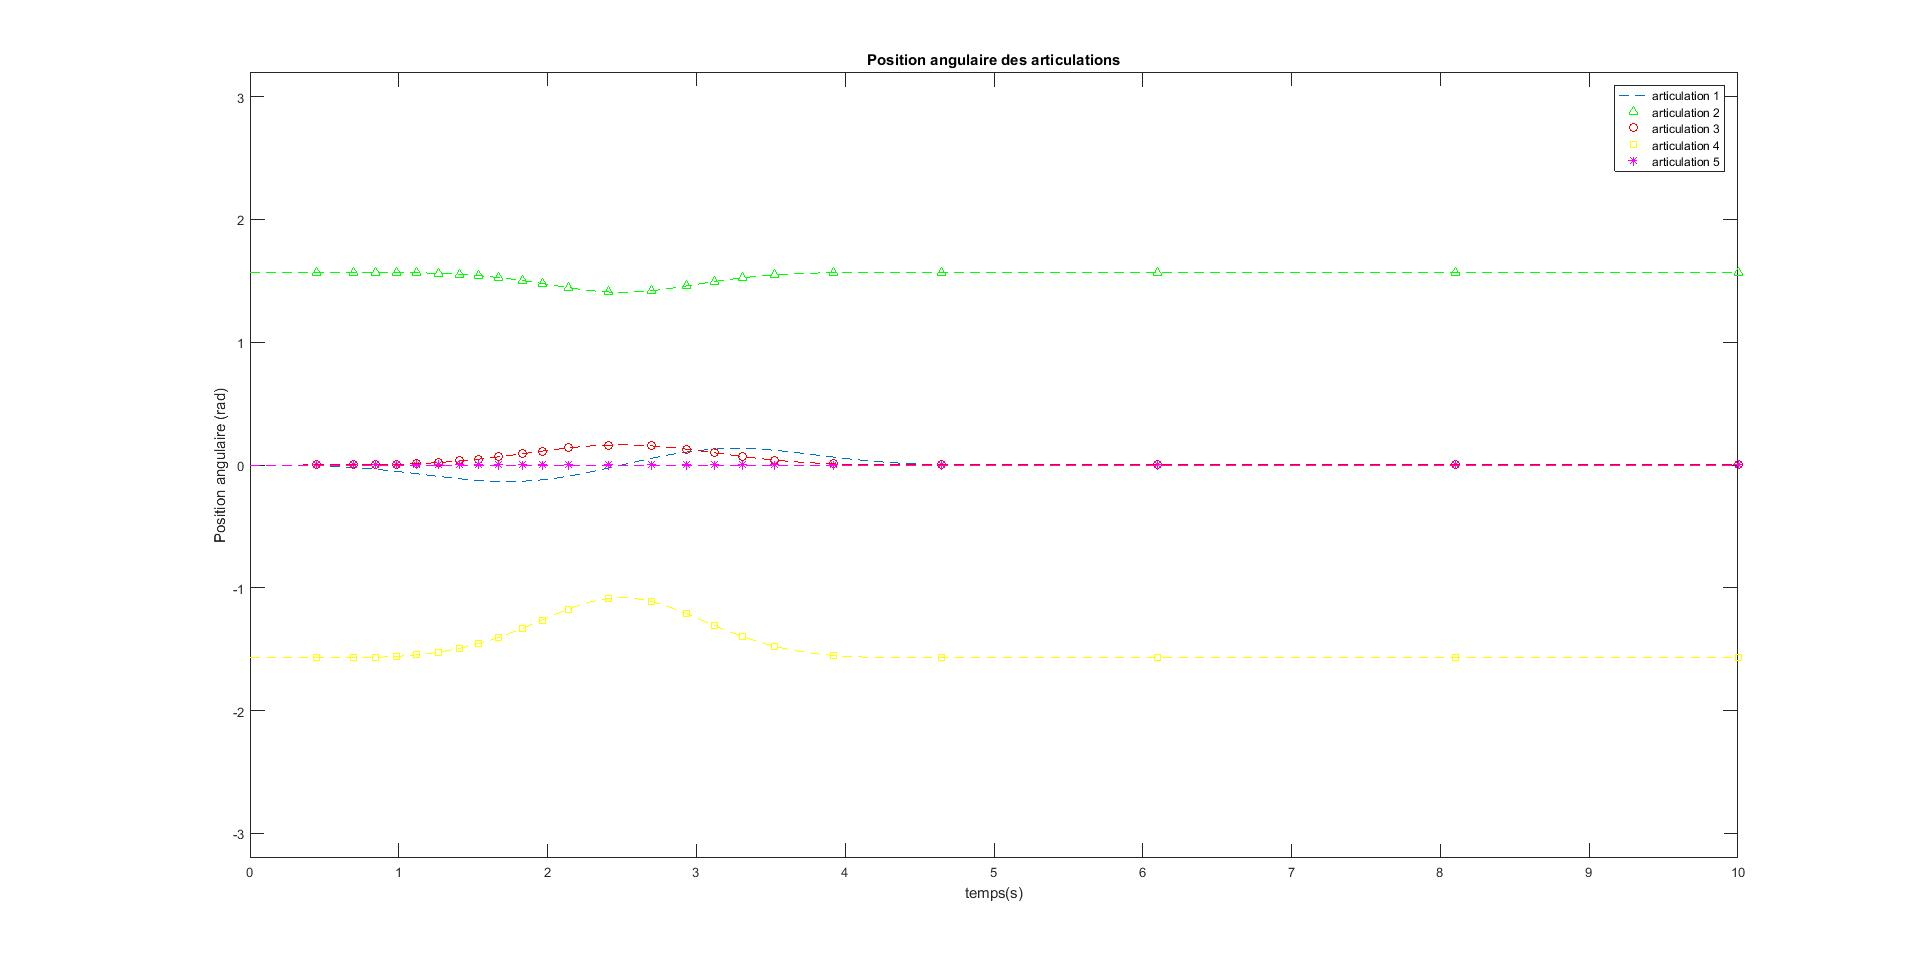
\includegraphics[width=\textwidth]{./Ctraj_positionAng_cascade.JPG}
		\caption{Réponse temporelle des positions angulaires des axes du robot commandé par la méthode cascade pour suivre une trajectoire circulaire}
		\label{fig:Ctraj_positionAng_cascade}
	\end{center}
\end{figure}
\newpage
\begin{figure}[H]
	\begin{center}
		\captionsetup{justification=centering,margin=1cm}	
		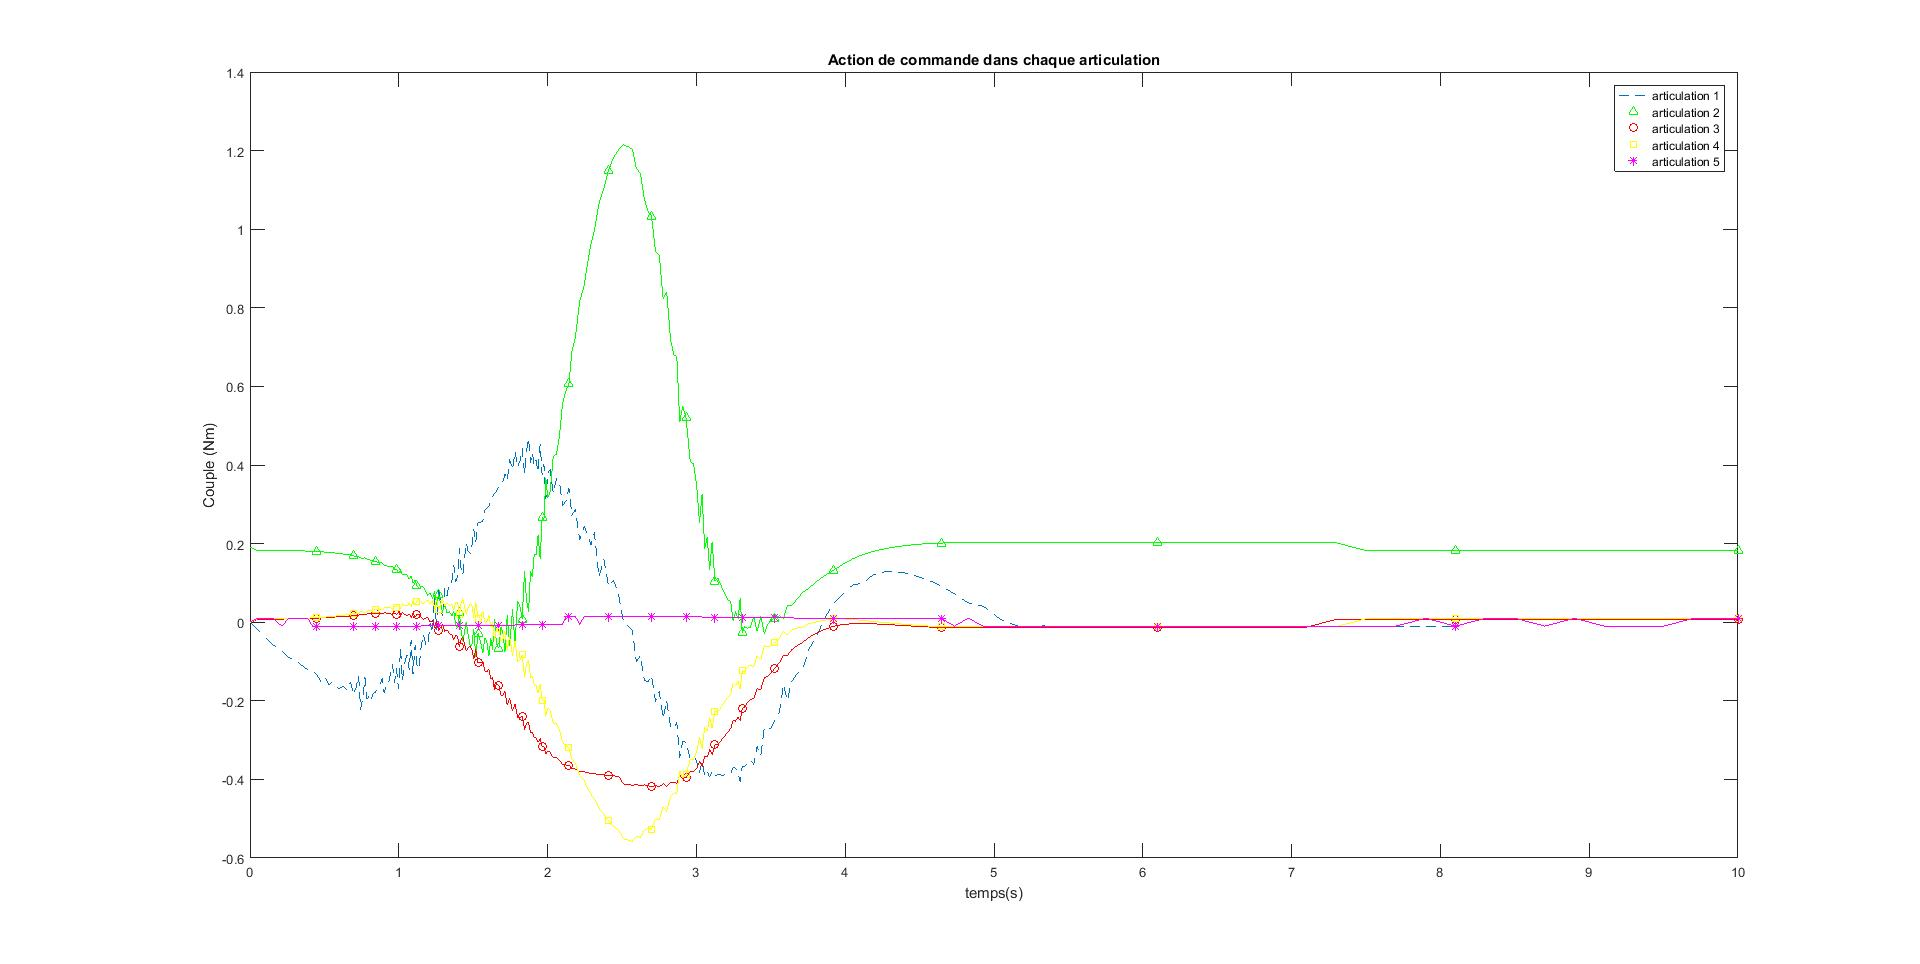
\includegraphics[width=\textwidth]{./Ctraj_commande_cascade.JPG}
		\caption{Efforts de commande appliqués aux articulations du robot commandé par la méthode cascade pour suivre une trajectoire circulaire}
		\label{fig:Ctraj_commande_cascade}
	\end{center}
\end{figure}


\textbf{Commande par MDI}
\newline

On a mis en \oe{}vre cette commande sur Matlab et Simulink en utilisant la commande PID angulaire qui était déjà près. Premièrement, on a besoin de convertir tous les trajectoires de l'espace articulaire à l'espace angulaire en utilisant le MDI. Ensuite, on peut utiliser ces trajectoires comme consignes pour la commande angulaire PID dévéloppée sur Simulink. Cela nous donne des résultats similaires pour ces deux méthodes de commande. Dans la suite, on a les graphiques de la réponse temporelle de la position de l'outil à une consigne de variation de position en échellon filtré par un système de premier ordre de valeur $ \left[0.1, 0, 0 \right] $, des positions angulaire des articulation et des efforts de commande.

\begin{figure}[H]
	\begin{center}	
		\captionsetup{justification=centering,margin=1cm}
		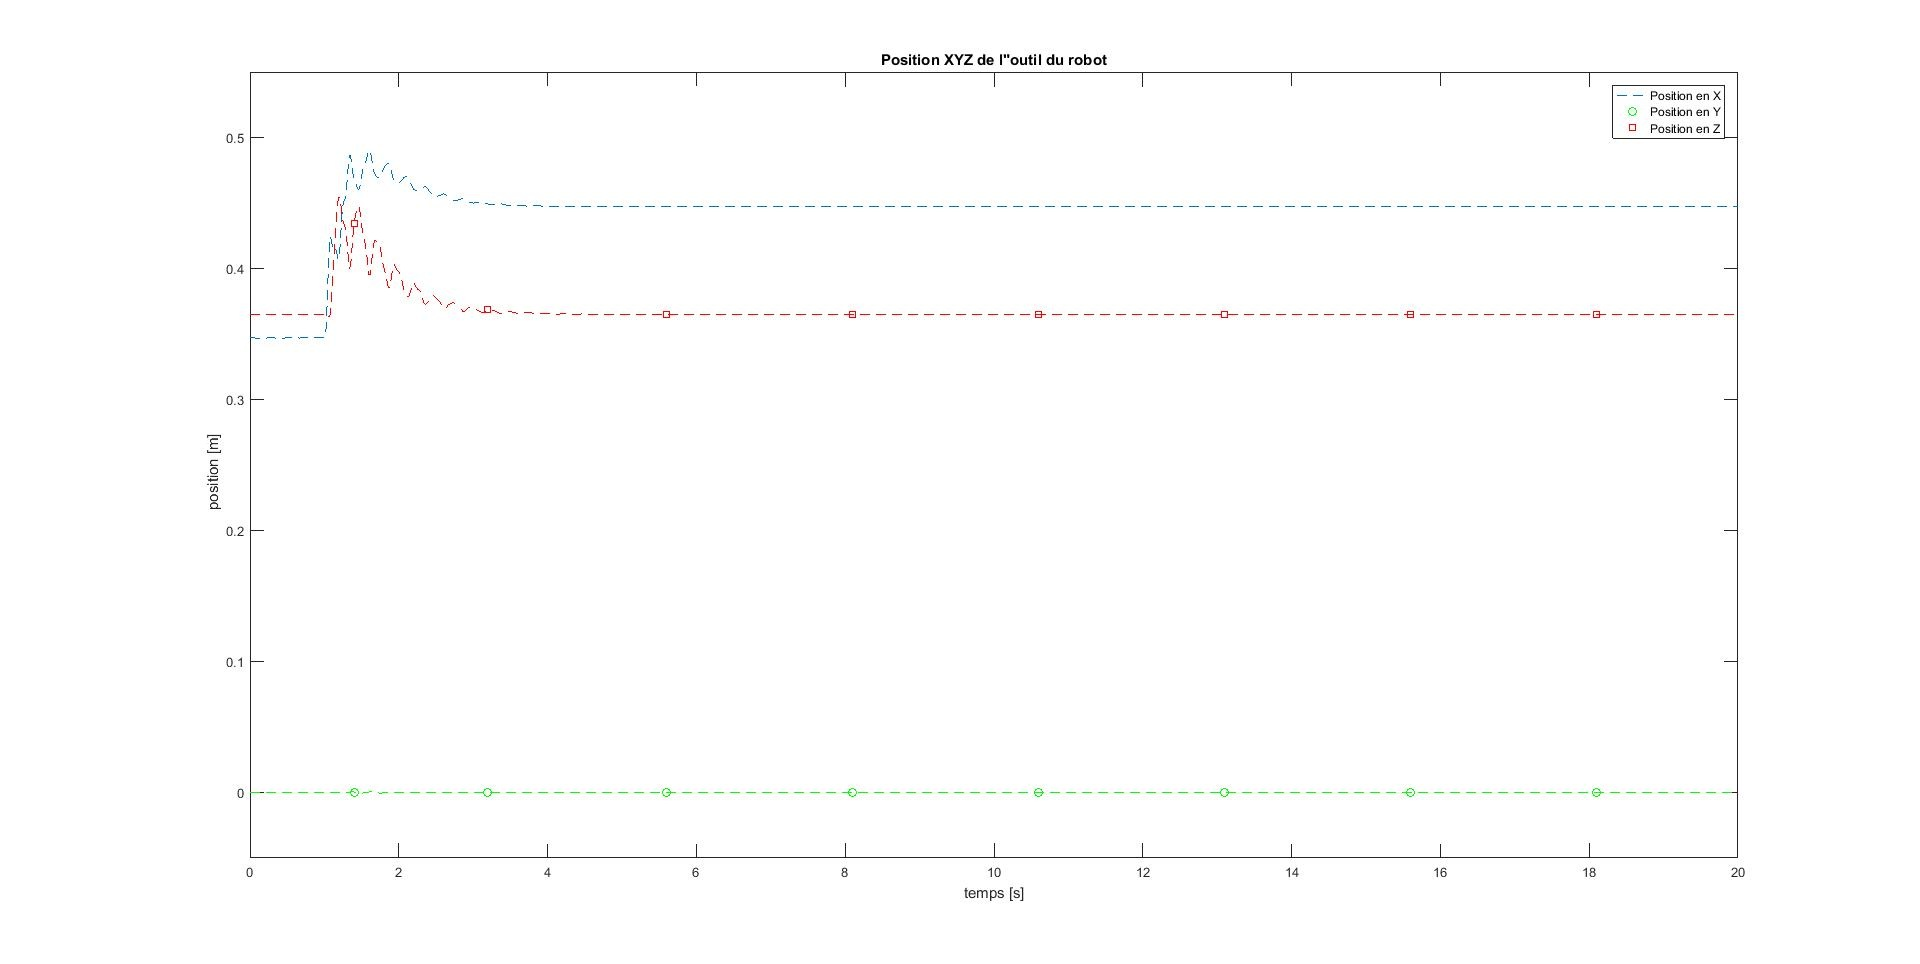
\includegraphics[width=\textwidth]{./res_positionLin_MDI.JPG}
		\caption{Réponse temporelle de la position de l'outil du robot commandé par le MDI et un PID articulaire à une consigne en échellon filtré}
		\label{fig:res_positionLin_MDI}
	\end{center}
\end{figure}

\begin{figure}[H]
	\begin{center}
		\captionsetup{justification=centering,margin=1cm}	
		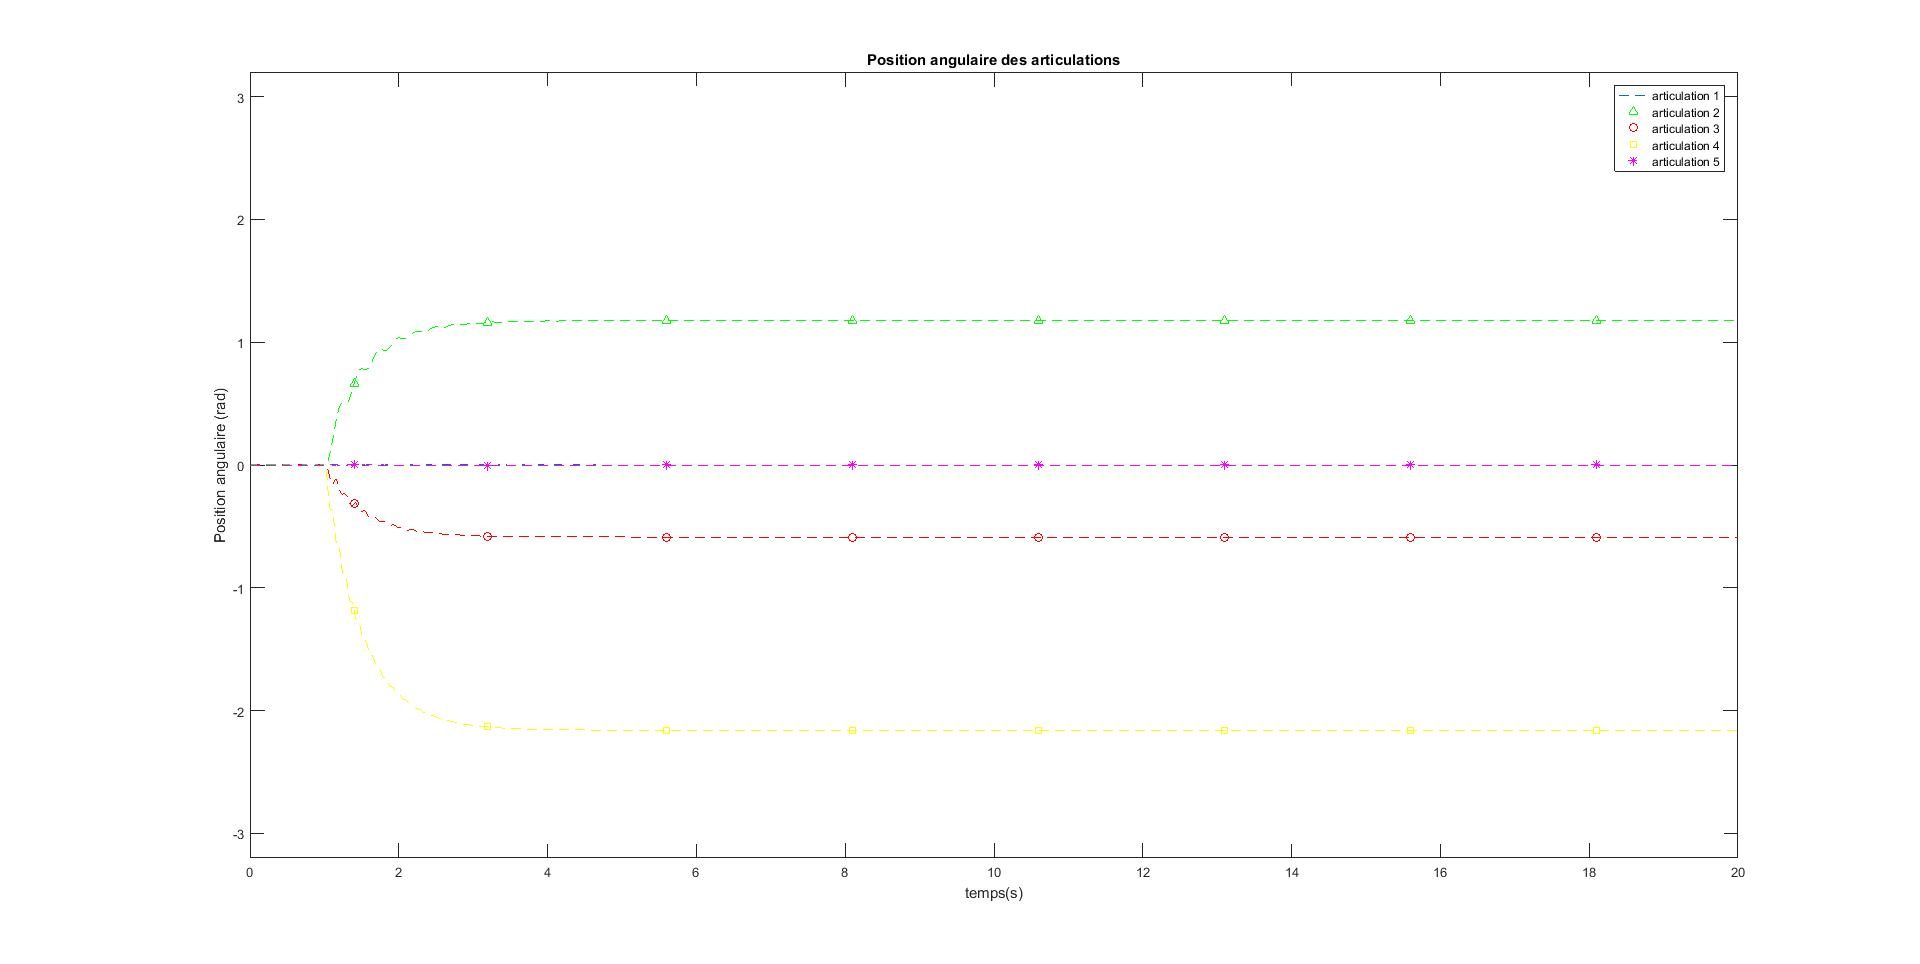
\includegraphics[width=\textwidth]{./res_positionAng_MDI.JPG}
		\caption{Réponse temporelle des positions angulaires des axes du robot commandé par le MDI et un PID articulaire à une consigne en échellon filtré}
		\label{fig:res_positionAng_MDI}
	\end{center}
\end{figure}

\begin{figure}[H]
	\begin{center}
		\captionsetup{justification=centering,margin=1cm}	
		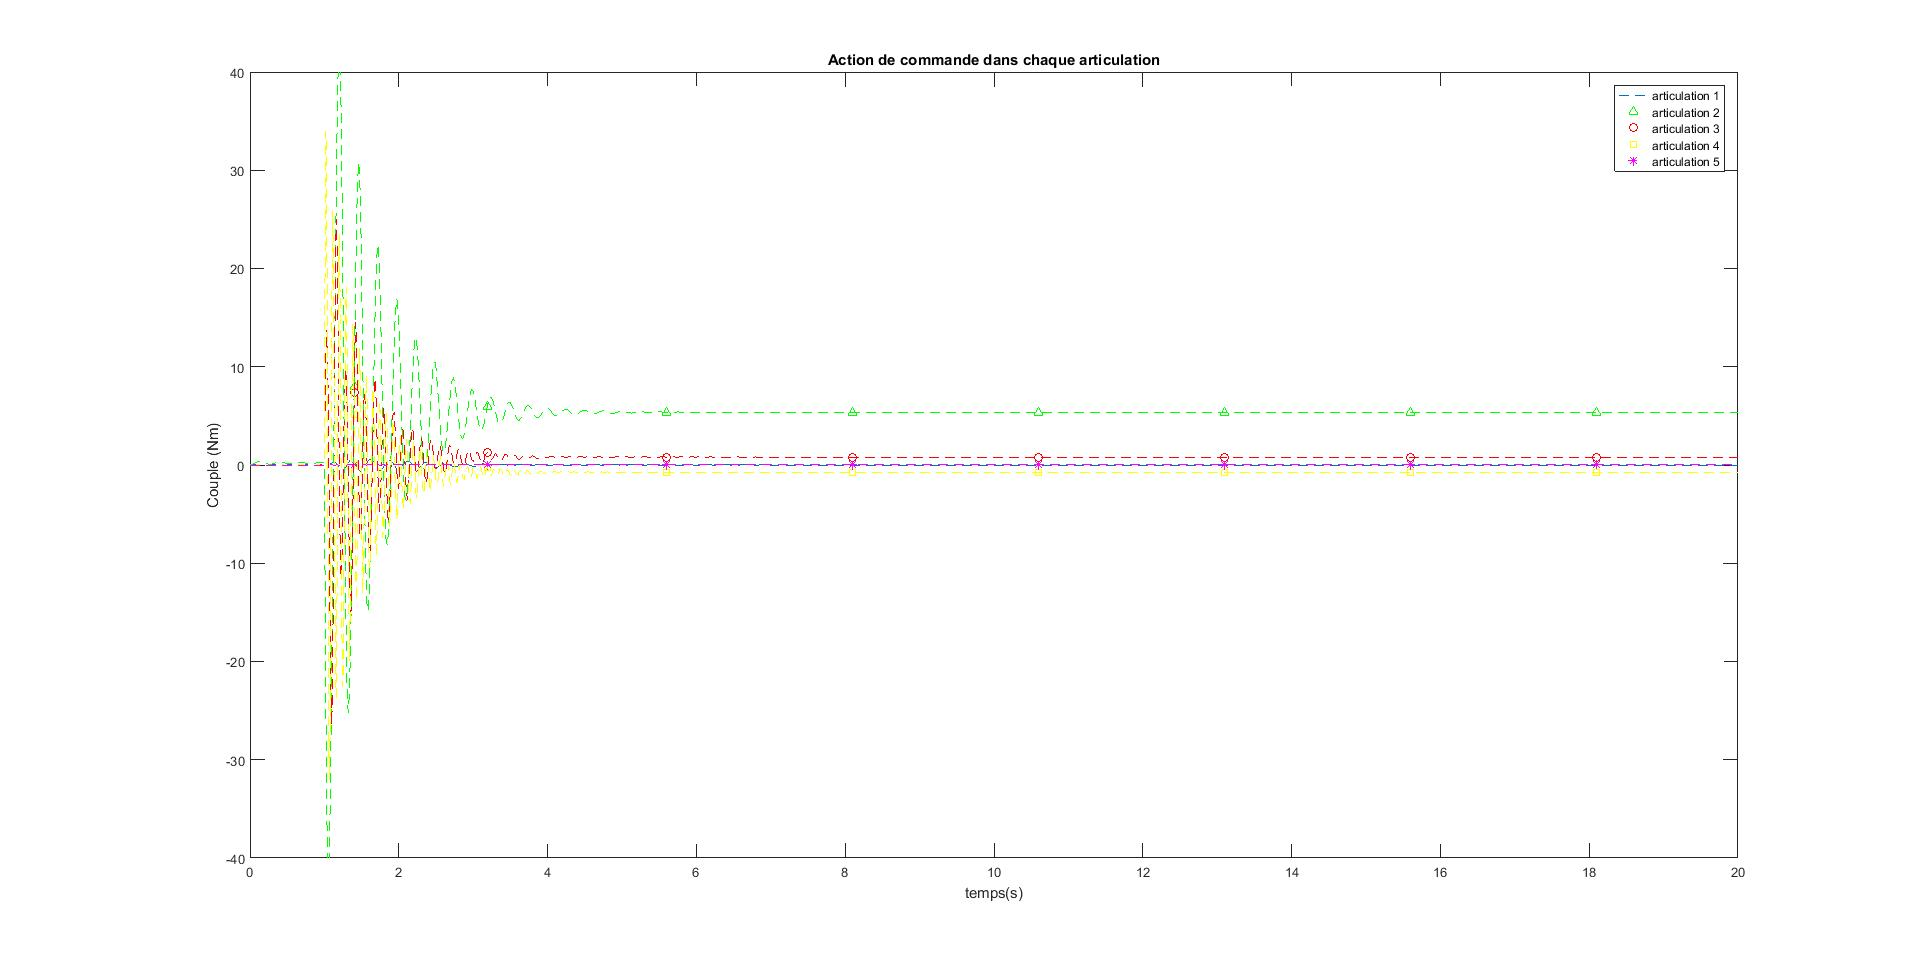
\includegraphics[width=\textwidth]{./res_commande_MDI.JPG}
		\caption{Efforts de commande appliqués aux articulations du robot commandé par le MDI et un PID articulaire à une consigne en échellon filtré}
		\label{fig:res_commande_MDI}
	\end{center}
\end{figure}

On observe dans ces graphiques que, au régime, le système suit bien la consigne, avec les positions angulaires stables et les efforts de commande que ne sont pas trop importants. Par contre, il y a beaucoup de fluctuation dans le transitoire, et les efforts de commande arrivent à des valeurs plus importantes. Cela était attendu une fois que ces fluctuations sont présentes aussi dans la commande angulaire PID.

Dans la suite, on a les réponses de ce système à des trajectoires linéaire et angulaire de consigne, qui répresent mieux la façon dont on veux que le robot se déplace dans notre application. 

\begin{figure}[H]
	\begin{center}	
		\captionsetup{justification=centering,margin=1cm}
		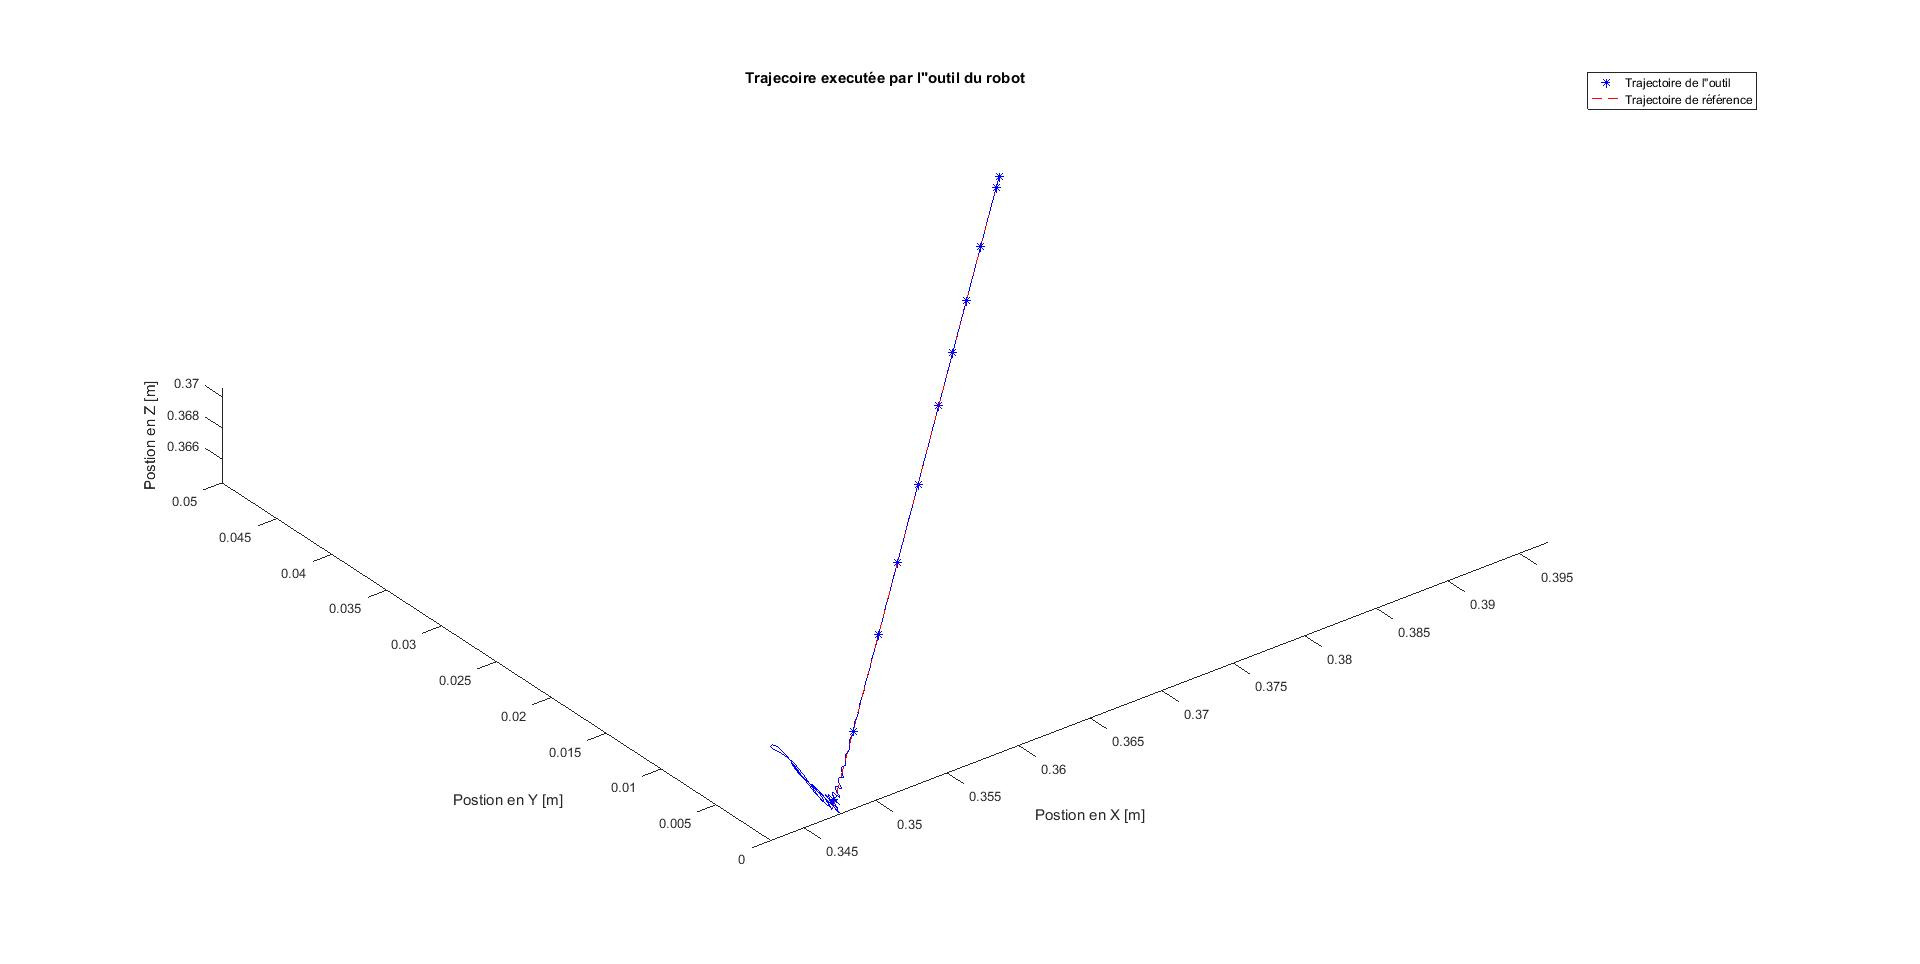
\includegraphics[width=\textwidth]{./Ltraj_positionLin_MDI.JPG}
		\caption{Comparaison de la trajectoire éxécutée par l'outil du robot commandé par le MDI et un PID angulaire et la trajectoire de référence linéaire}
		\label{fig:Ltraj_positionLin_MDI}
	\end{center}
\end{figure}

\begin{figure}[H]
	\begin{center}	
		\captionsetup{justification=centering,margin=1cm}
		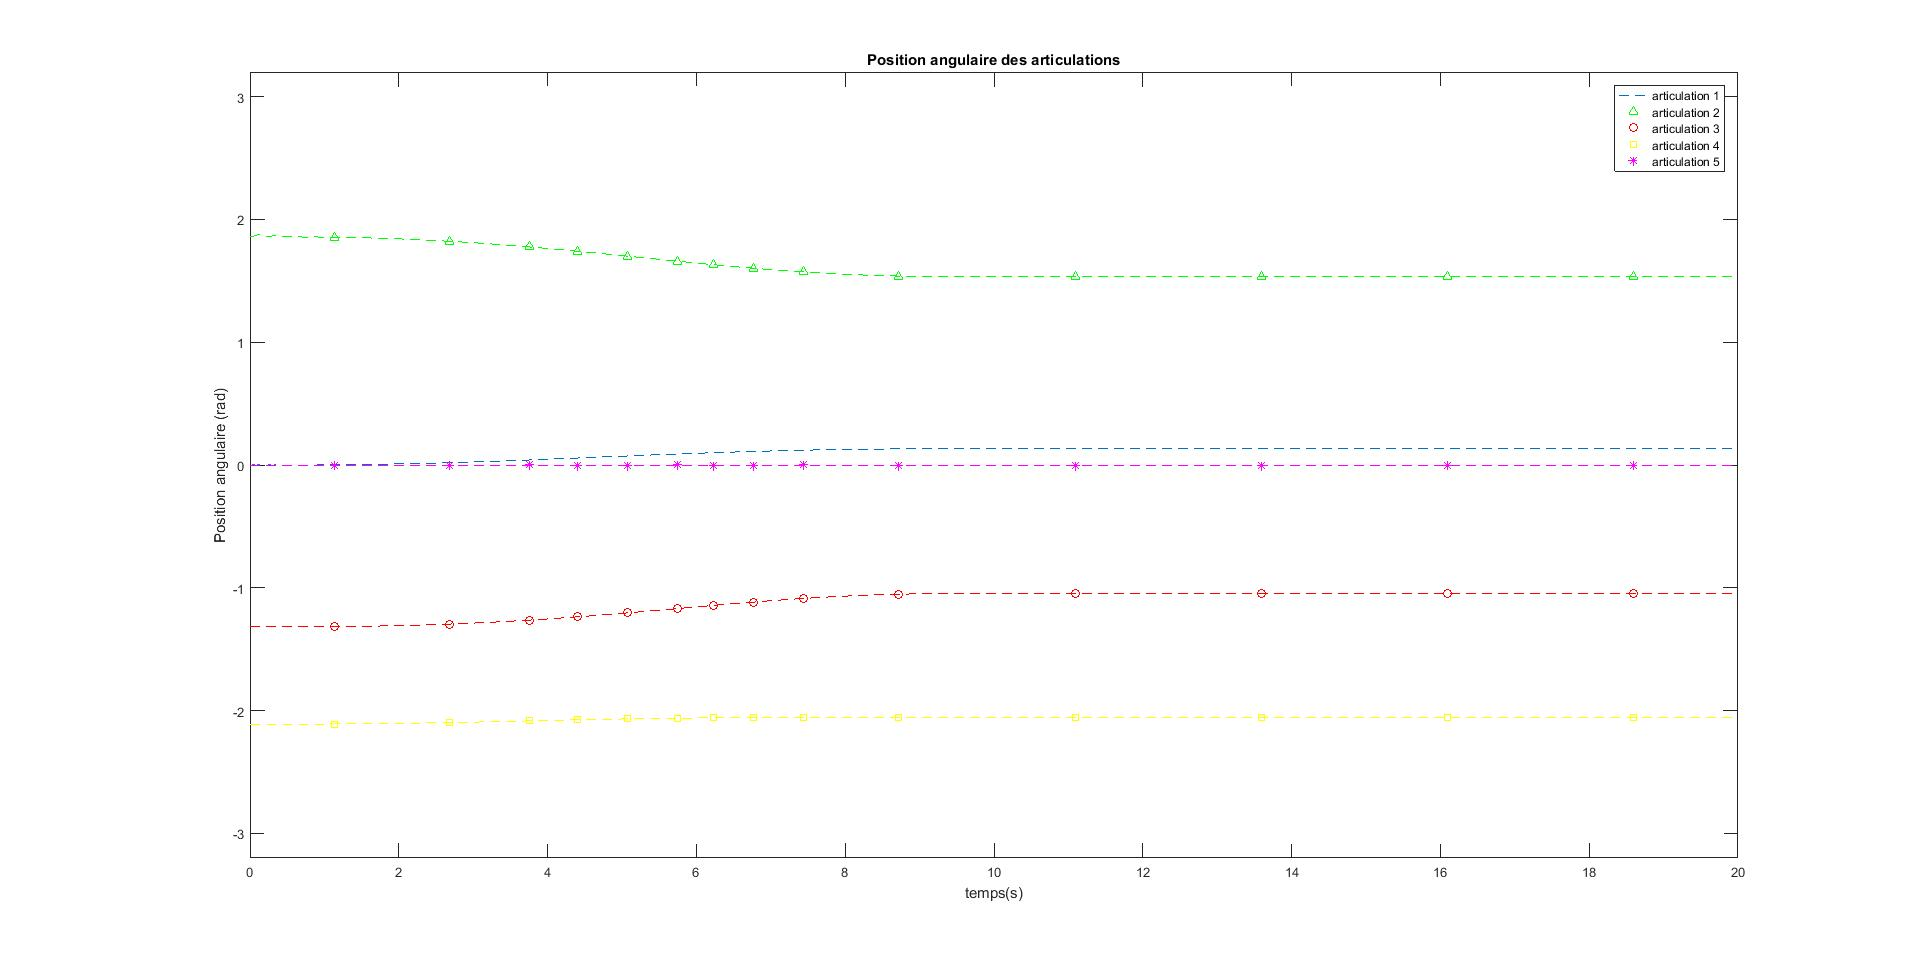
\includegraphics[width=\textwidth]{./Ltraj_positionAng_MDI.JPG}
		\caption{Réponse temporelle des positions angulaires des axes du robot commandé par le MDI et un PID angulaire pour suivre une trajectoire linéaire}
		\label{fig:Ltraj_positionAng_MDI}
	\end{center}
\end{figure}
\newpage
\begin{figure}[H]
	\begin{center}
		\captionsetup{justification=centering,margin=1cm}	
		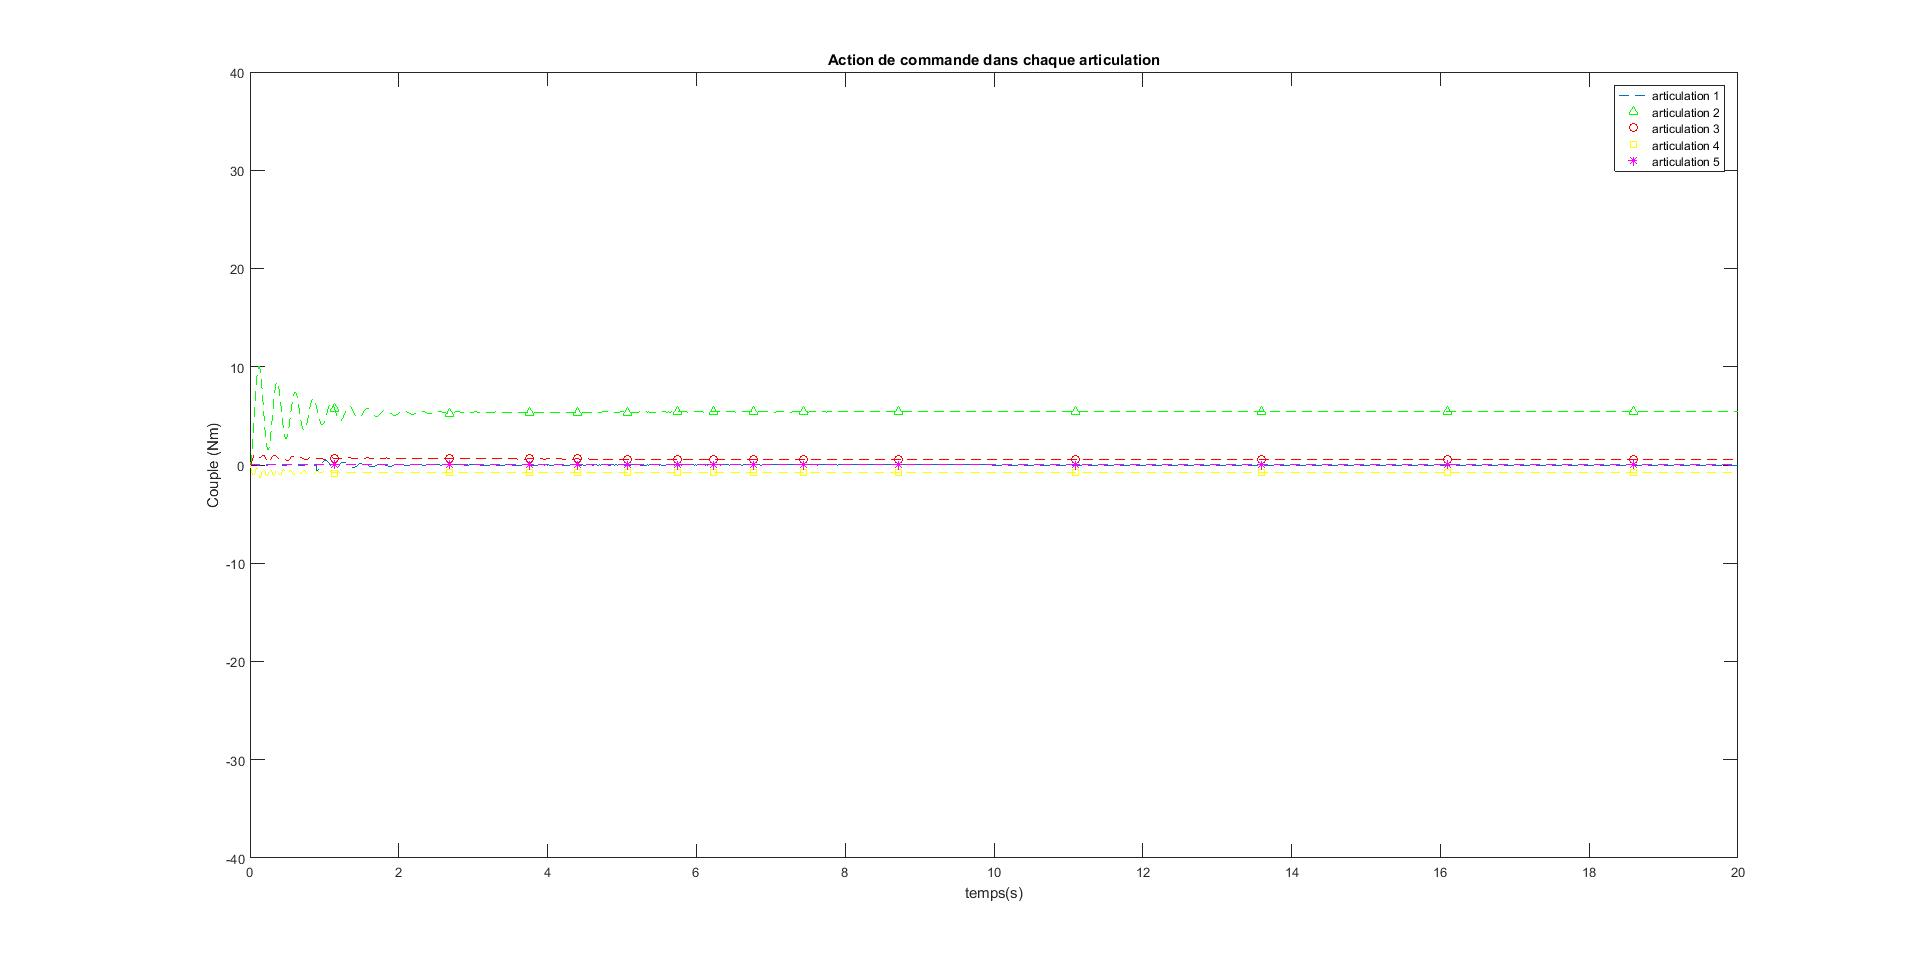
\includegraphics[width=\textwidth]{./Ltraj_commande_MDI.JPG}
		\caption{Efforts de commande appliqués aux articulations du robot commandé par le MDI et un PID angulaire pour suivre une trajectoire linéaire}
		\label{fig:Ltraj_commande_MDI}
	\end{center}
\end{figure}

\begin{figure}[H]
	\begin{center}	
		\captionsetup{justification=centering,margin=1cm}
		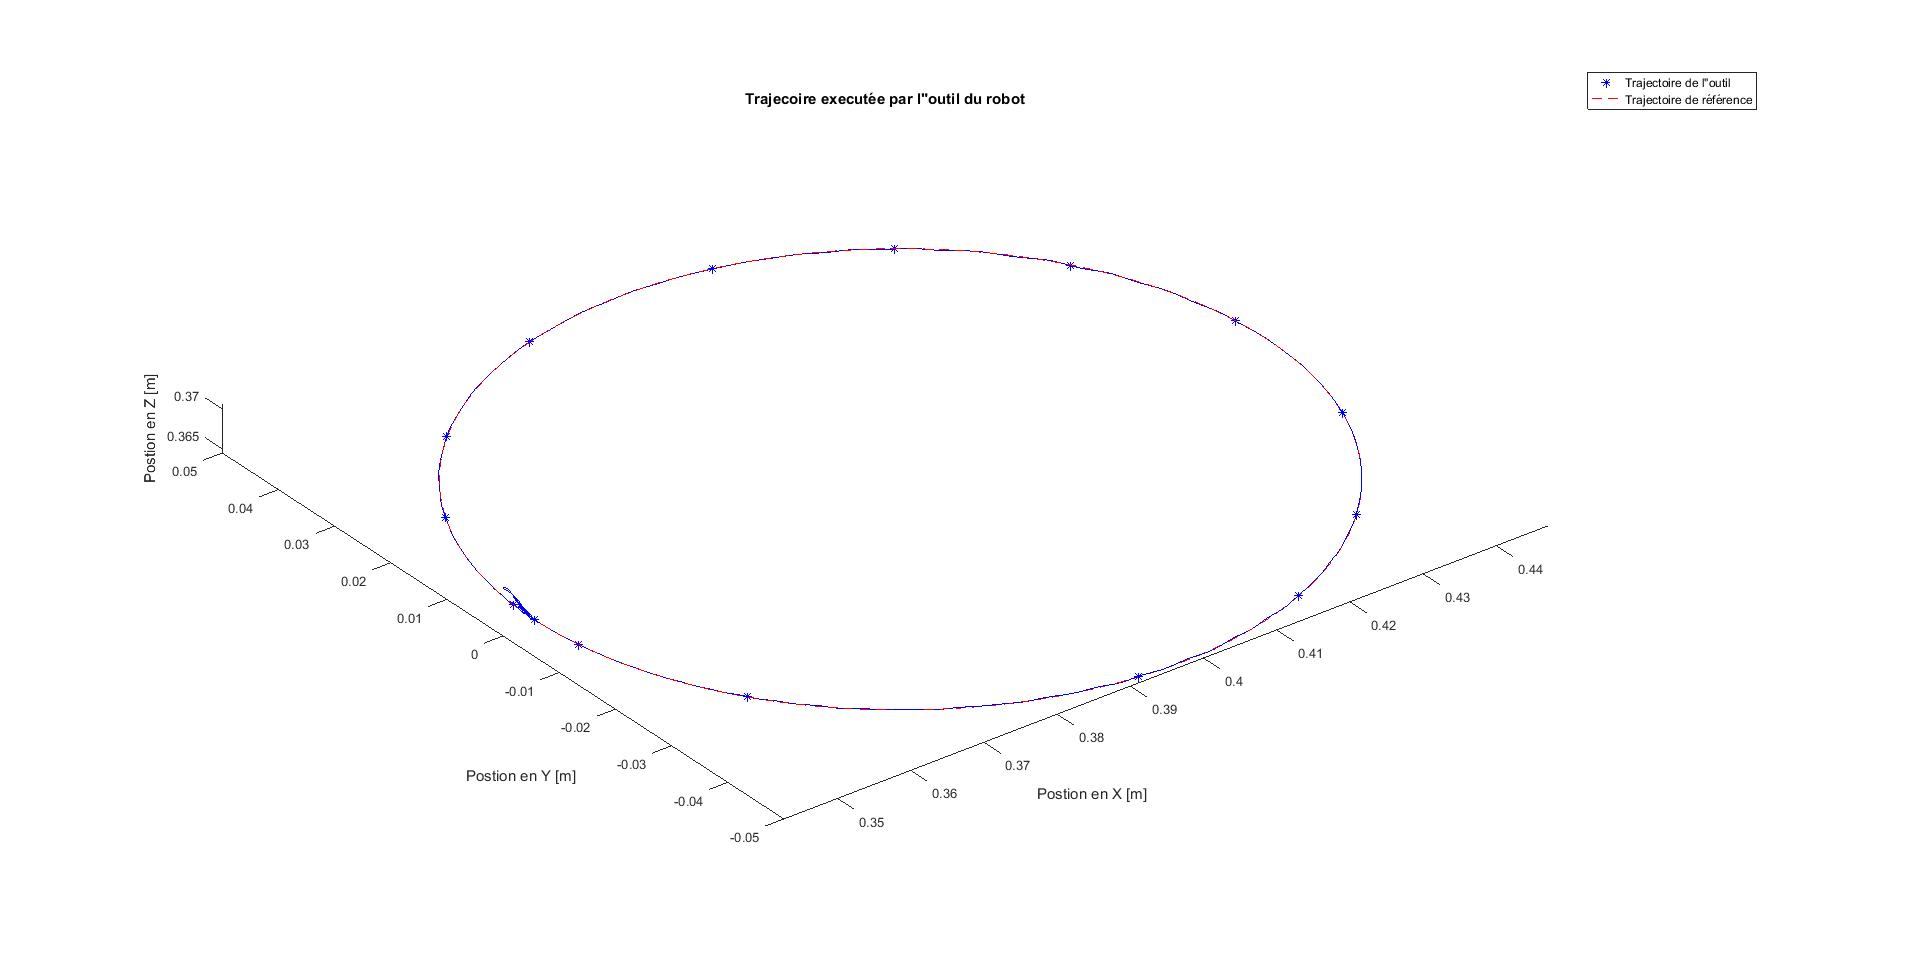
\includegraphics[width=\textwidth]{./Ctraj_positionLin_MDI.JPG}
		\caption{Comparaison de la trajectoire éxécutée par l'outil du robot commandé par le MDI et un PID angulaire et la trajectoire de référence circulaire}
		\label{fig:Ctraj_positionLin_MDI}
	\end{center}
\end{figure}
\newpage
\begin{figure}[H]
	\begin{center}	
		\captionsetup{justification=centering,margin=1cm}
		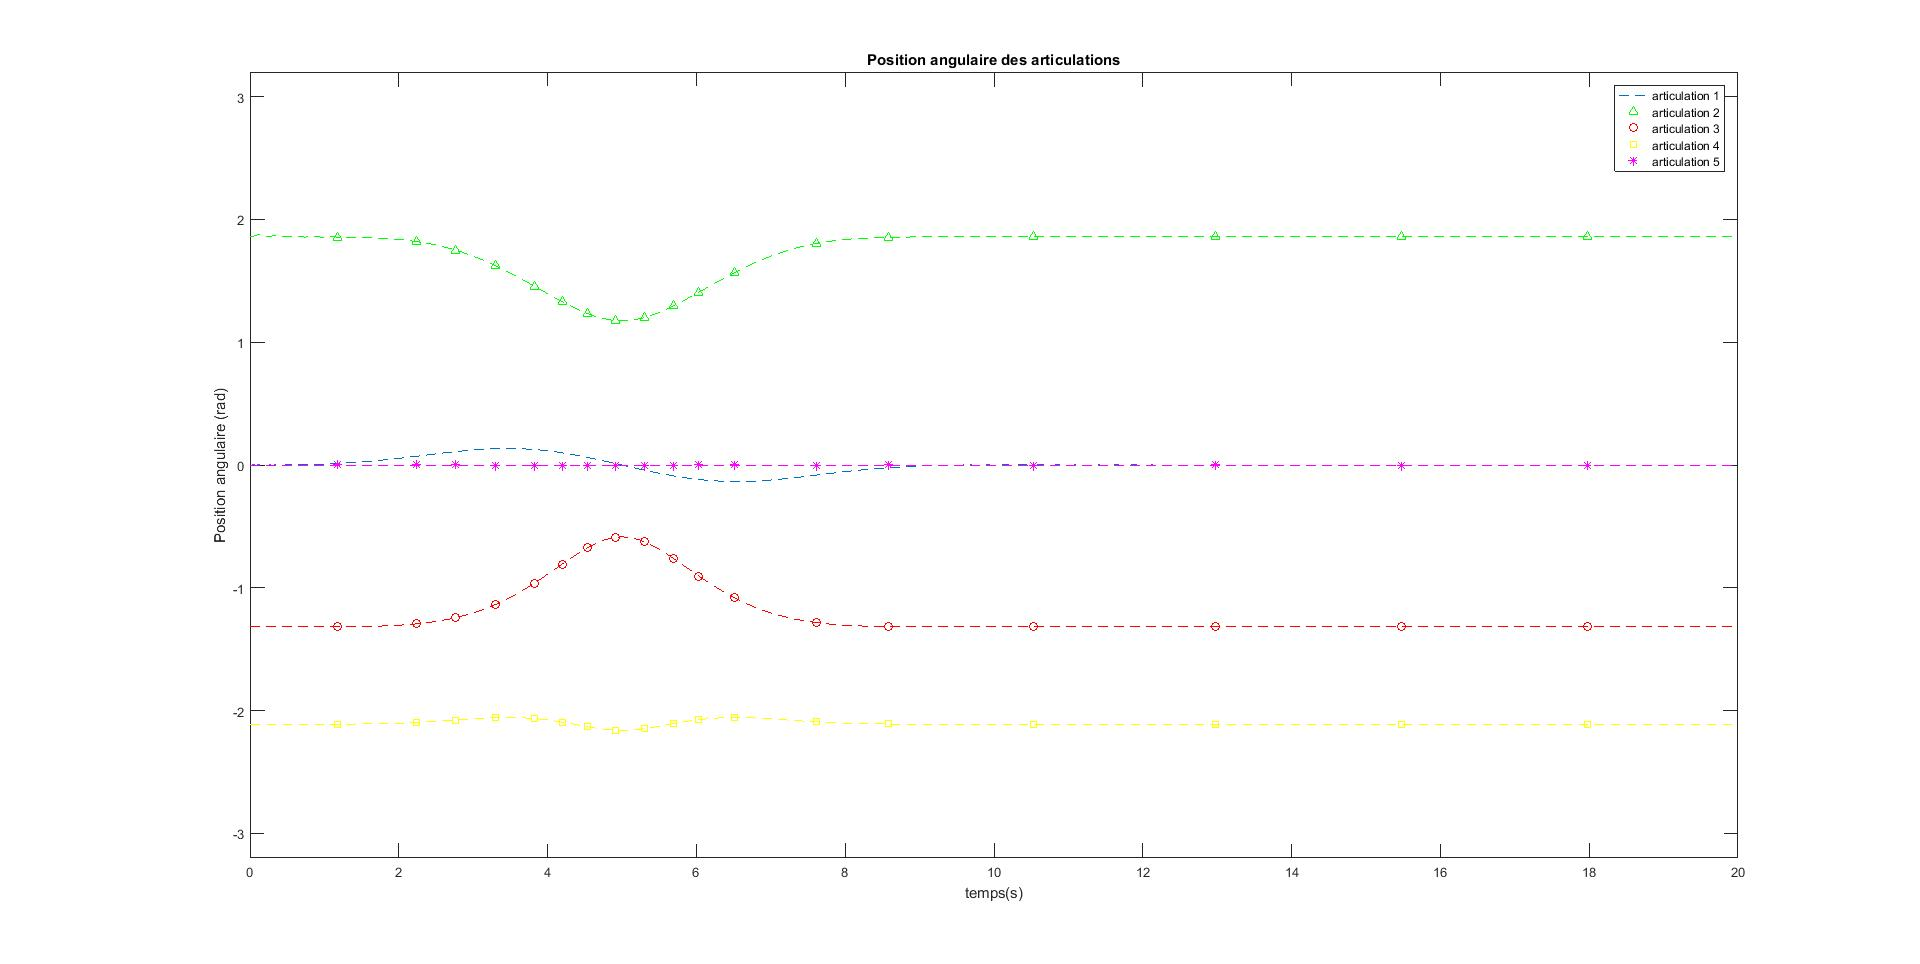
\includegraphics[width=\textwidth]{./Ctraj_positionAng_MDI.JPG}
		\caption{Réponse temporelle des positions angulaires des axes du robot commandé par le MDI et un PID angulaire pour suivre une trajectoire circulaire}
		\label{fig:Ctraj_positionAng_MDI}
	\end{center}
\end{figure}

\begin{figure}[H]
	\begin{center}	
		\captionsetup{justification=centering,margin=1cm}
		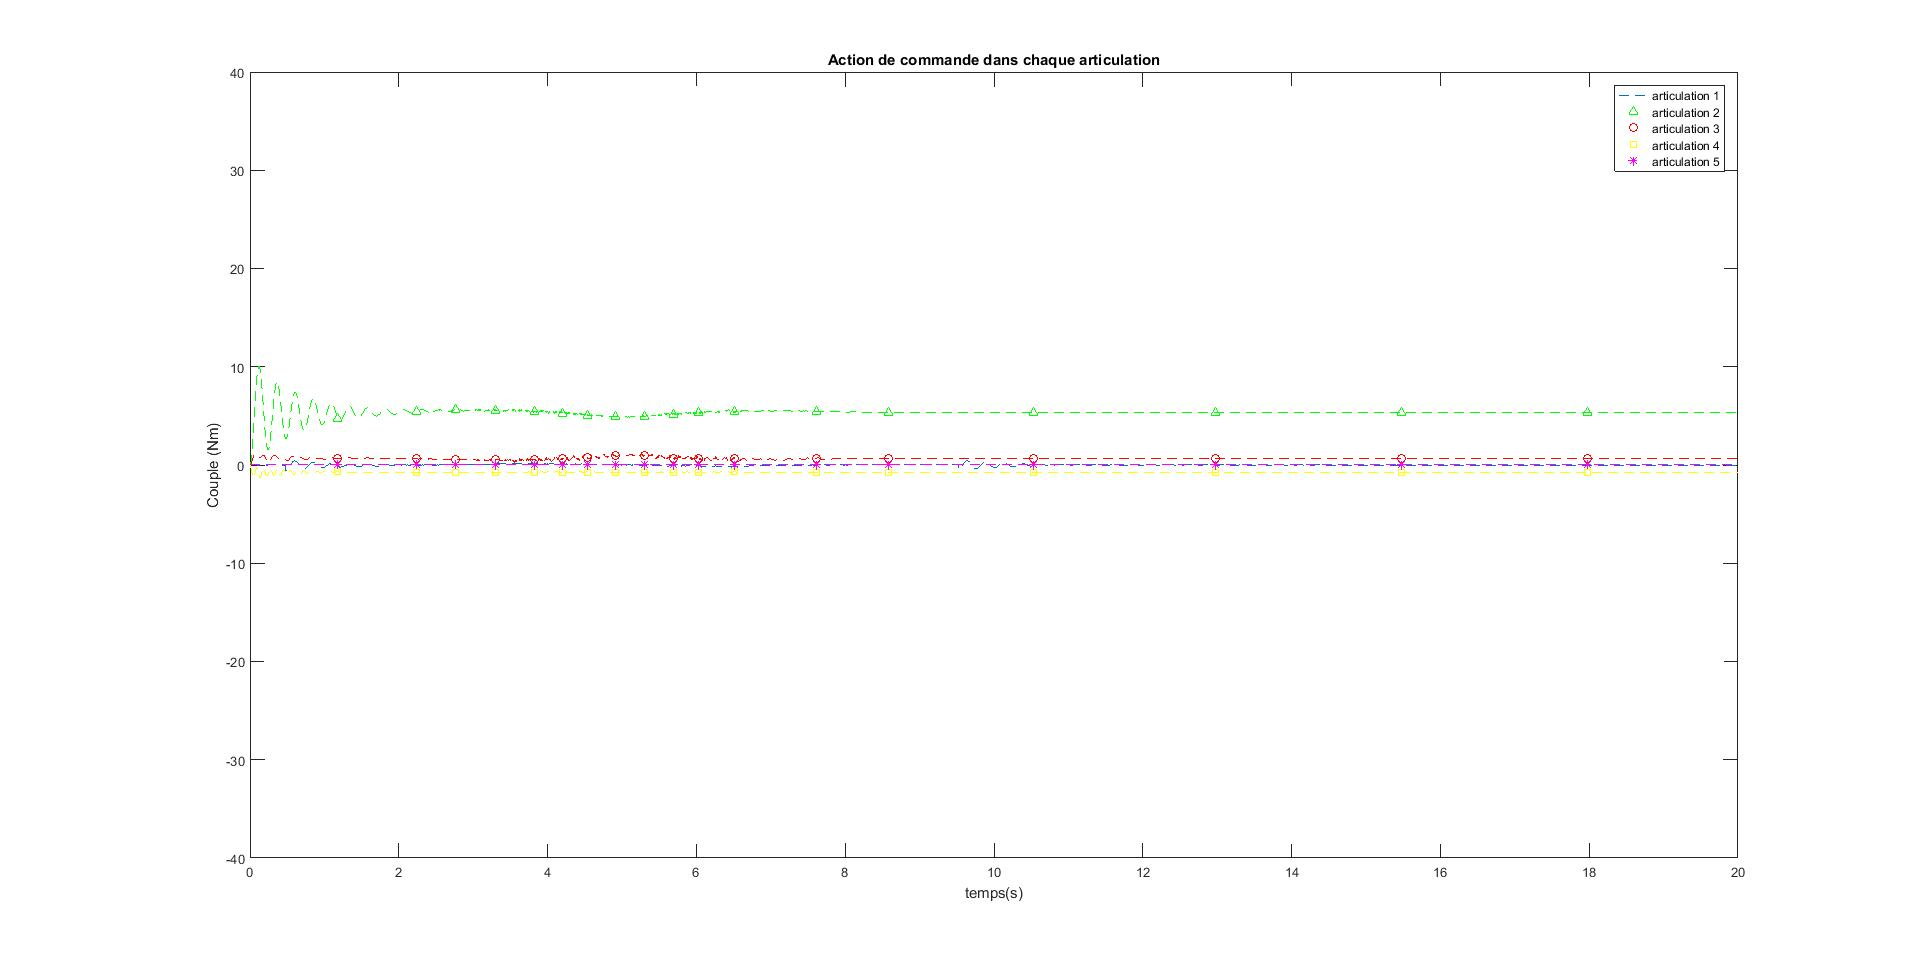
\includegraphics[width=\textwidth]{./Ctraj_commande_MDI.JPG}
		\caption{Efforts de commande appliqués aux articulations du robot commandé par le MDI et un PID angulaire pour suivre une trajectoire circulaire}
		\label{fig:Ctraj_commande_MDI}
	\end{center}
\end{figure}

On peut noter que le système suivre bien les deux types de trajectoire, avec des variations angulaires qui sont lisses et stabilisent bien après le mouvement et avec des efforts de commande qui ne sont pas trop importants. Le seul problème sont des fluctuations qui apparaissent au début du déplacement, assoicées aux fluctuations dans les efforts de commande. En dépit d'être de petit amplitude (de l'ordre de 5mm), ces fluctuations peuvent gêner le mouvement du robot. Un meilleur réglage du PID est nécessaire pour réduire ces problèmes. 

On a dit dans la section \ref{Comm_Cart} qui cette méthode de commande prend en compte aussi l'orientation de l'outil et que pour un robot de 5 axes, une fois fixée la position, il ne sont faisables que les orientations dans lequelles l'axe Z du repère associé à l'outil est contenu dans le plan du bras du robot. Pour résoudre ce problème, on a decidé de faire les trajectoires avec l'outil tourné vers l'avant. En conséquence, il est nécessaire une étape au début du Jeu pour mettre le robot dans la même position initialle mais avec l'orientation désirée. On peut après laisser le robot pendant tout le jeu avec cette orientation. Dans la suite, on a les graphiques avec les réponses obtenues pour cette étape de orientation de l'outil.

\begin{figure}[H]
	\begin{center}
		\captionsetup{justification=centering,margin=1cm}	
		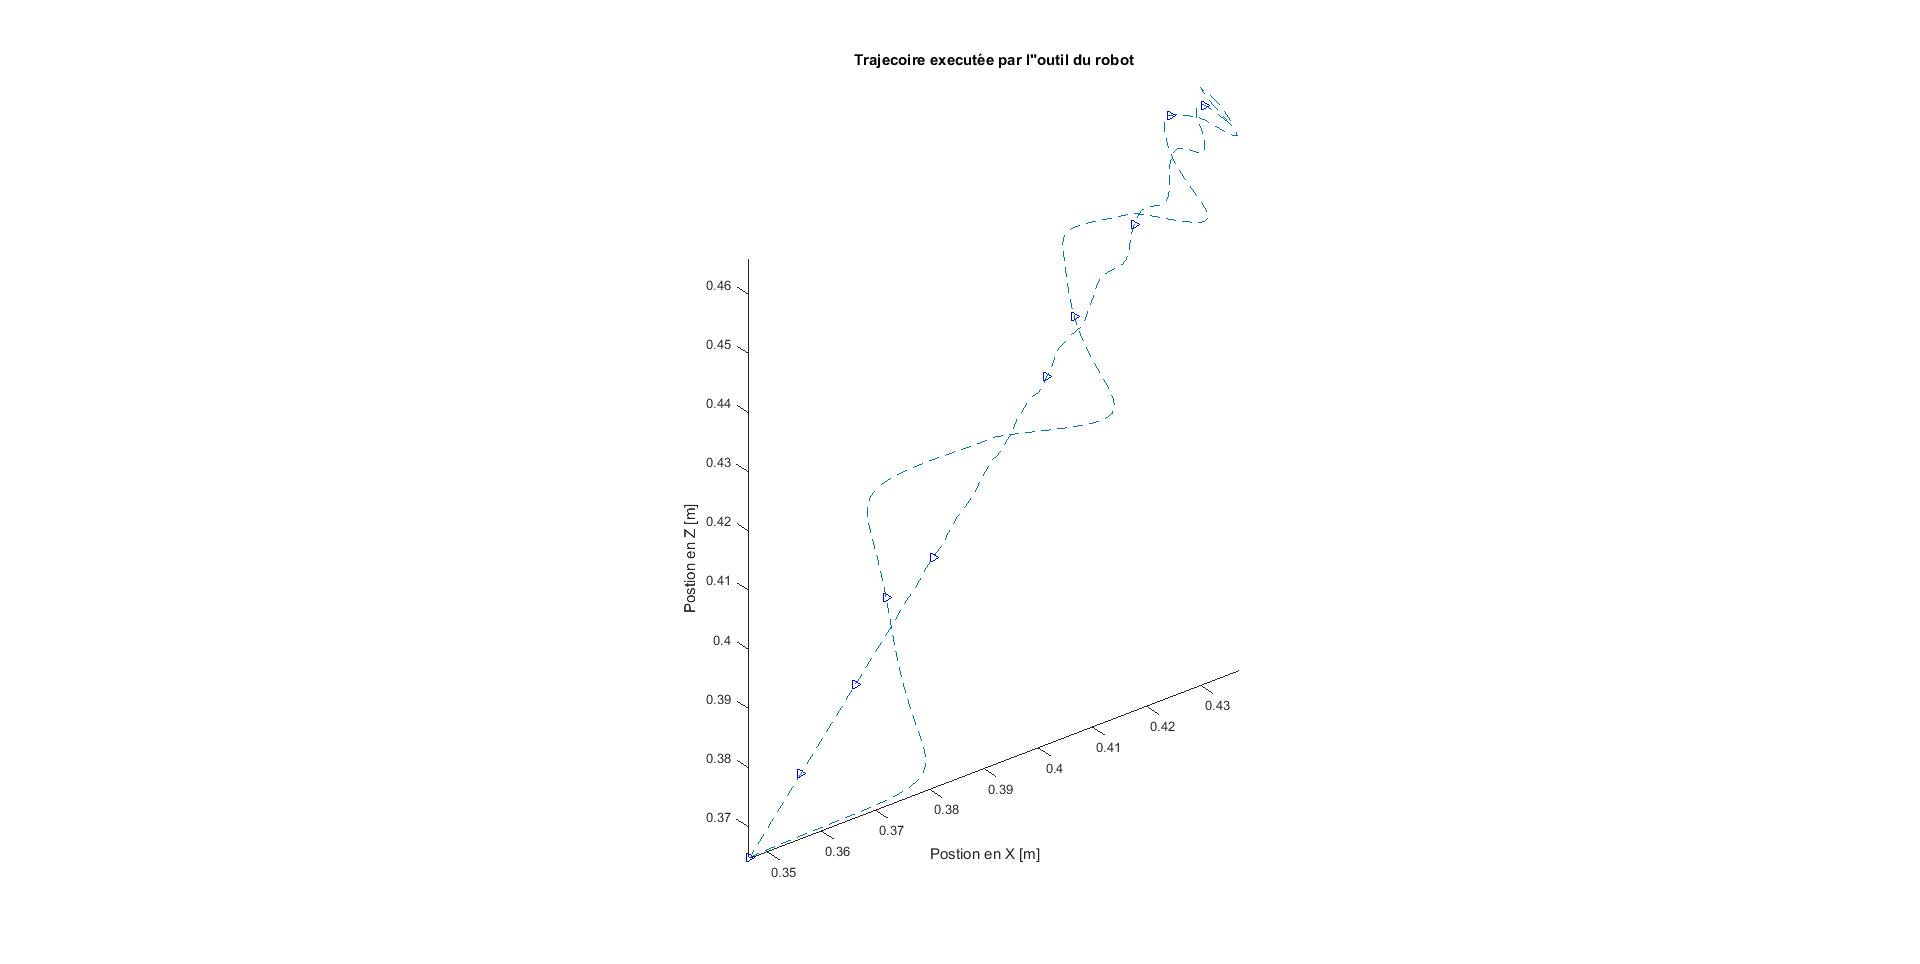
\includegraphics[width=\textwidth]{./Or_positionLin_MDI.JPG}
		\caption{Trajectoire éxécutée par l'outil du robot commandé par le MDI et un PID angulaire dans l'étape de orientation de l'outil}
		\label{fig:Or_positionLin_MDI}
	\end{center}
\end{figure}

\begin{figure}[H]
	\begin{center}
		\captionsetup{justification=centering,margin=1cm}	
		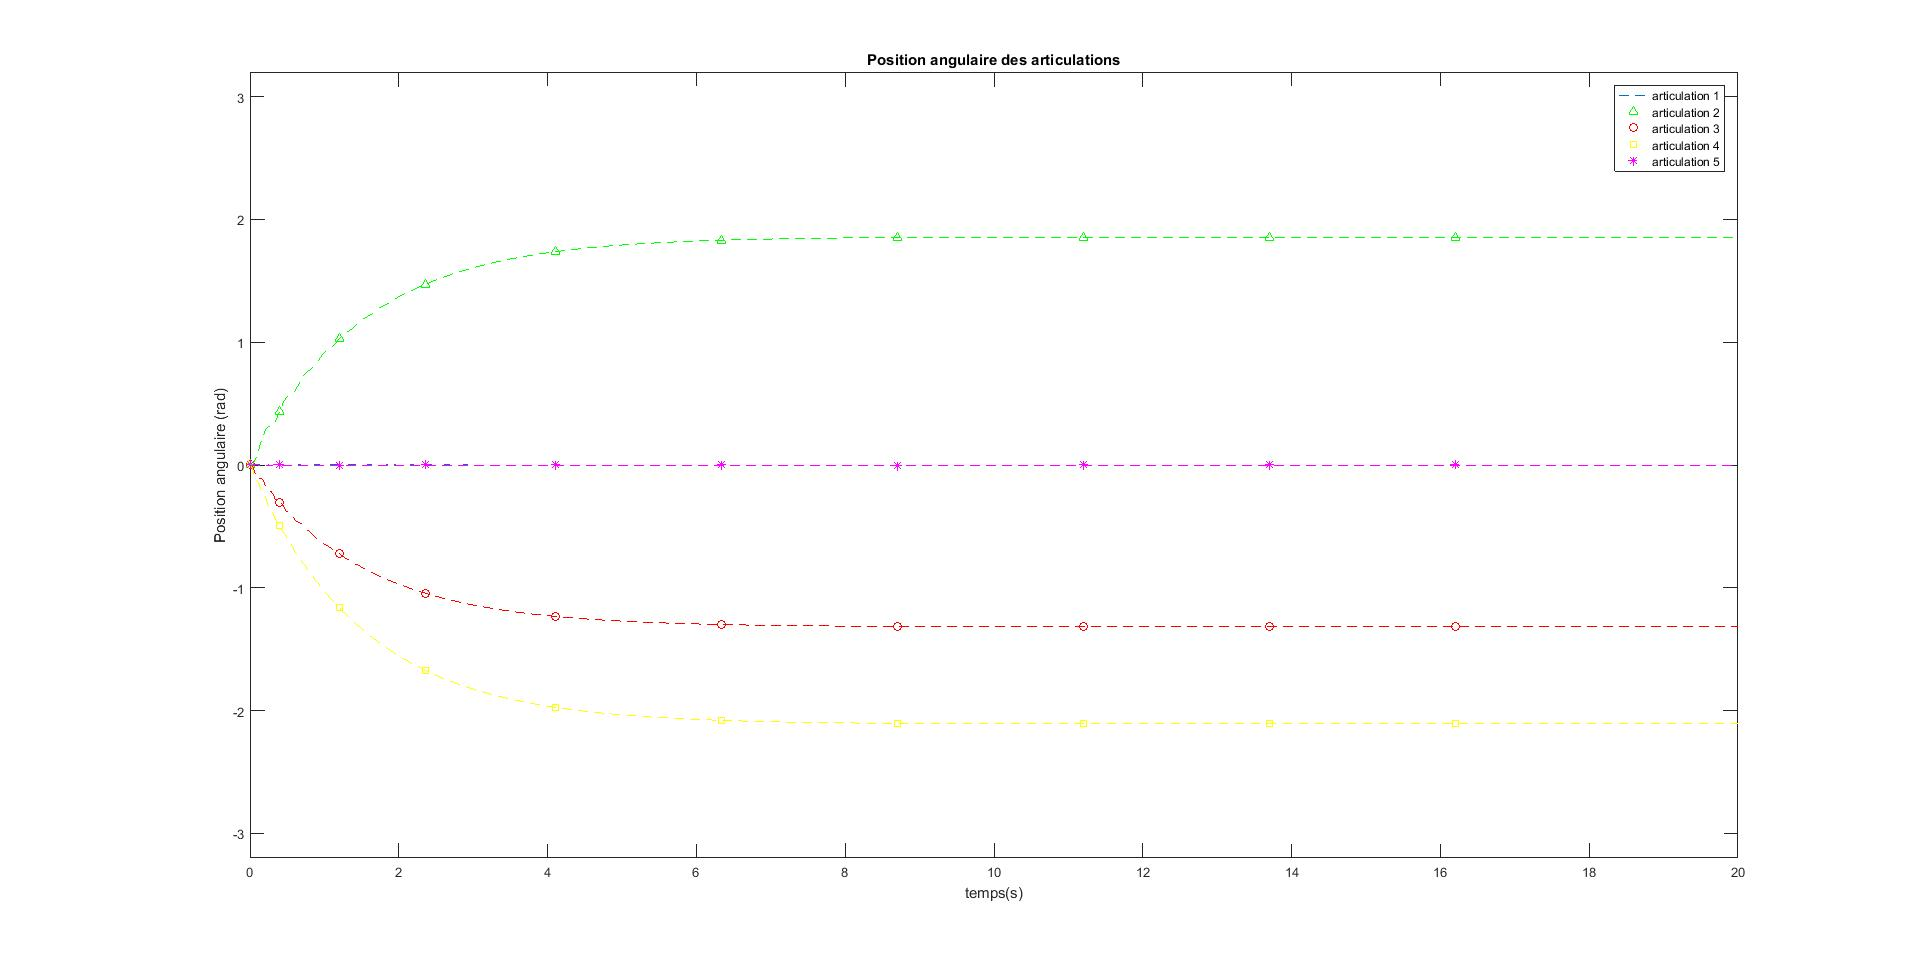
\includegraphics[width=\textwidth]{./Or_positionAng_MDI.JPG}
		\caption{Réponse temporelle des positions angulaires des axes du robot commandé par le MDI et un PID angulaire dans l'étape de orientation de l'outil}
		\label{fig:Or_positionAng_MDI}
	\end{center}
\end{figure}
\newpage
\begin{figure}[H]
	\begin{center}
		\captionsetup{justification=centering,margin=1cm}	
		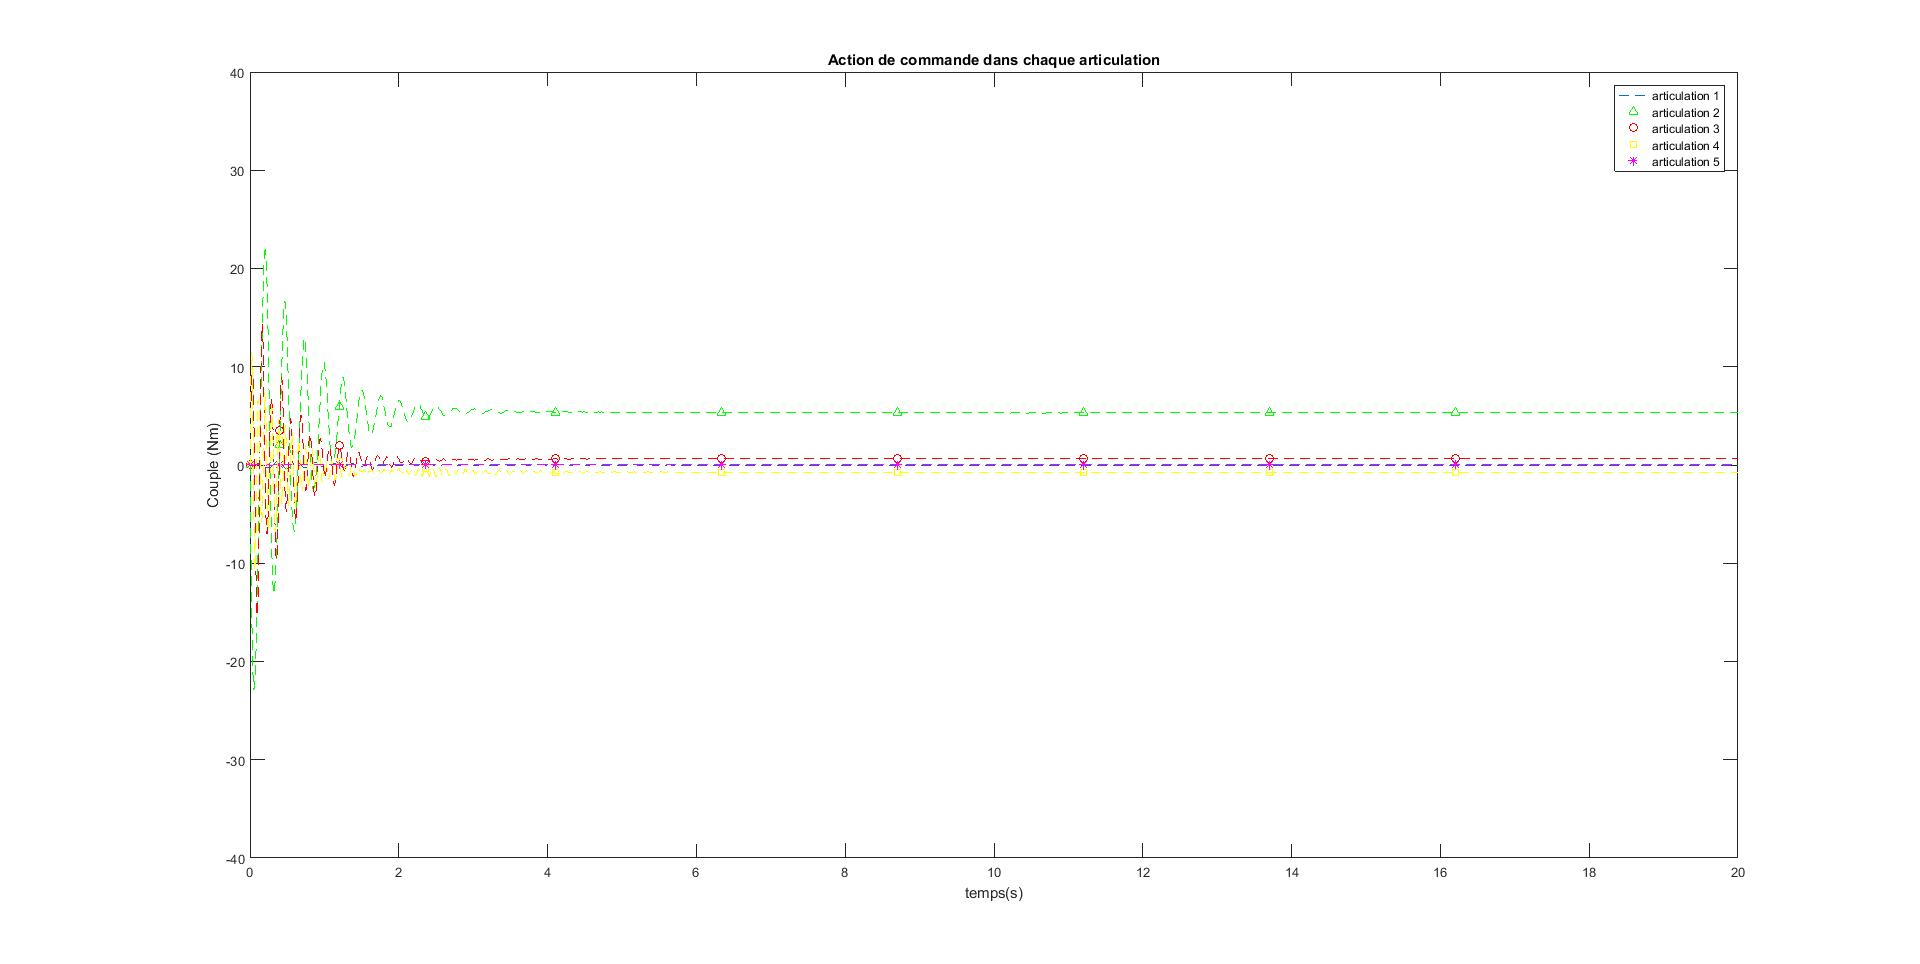
\includegraphics[width=\textwidth]{./Or_control_MDI.JPG}
		\caption{Efforts de commande appliqués aux articulations du robot commandé par le MDI et un PID angulaire dans l'étape de orientation de l'outil}
		\label{fig:Or_commande_MDI}
	\end{center}
\end{figure}

On observe que le robot retourne bien au point initial après un déplacement d'environ 14cm, les réponses des positions angulaires des axes sont lisses et les efforts de commande apliqués ne sont pas trop importants, malgré les fluctuations au début dues à une réglage insuffisante du PID angulaire.
\newline

\textbf{Commande PID Cartésienne}
\newline

On a essayé aussi de faire la commande du robot dans l'espace opérationnel avec juste un PID. Cette méthode est le plus simple sur le plan conceptuel, par contre il est vraiment difficile de le mettre en \oe{}uvre parce que il n'y a pas de méthode pour régler le PID, une fois que les équations qui décrivent le système sont non-linéaires et bien accouplé. 

Dans la suite, on montre les réponse obtenues par cette méthode avec une consigne de variation de position de $ \left[X,Y,Z\right] $ = $ \left[0.2, 0.2, -0.1\right] $ en échelon filtré par un système de premier ordre de constante de temps de 0.5s.

Premièrement, le robot n'arrive pas exactement á la consigne donnée, il reste toujours une erreur en régime permanent. De plus, le système est trop lente: il prend presque 7s pour arriver au régime, contre 2s des méthodes précédentes. Les positions angulaires et les efforts de contrôlen'arrivent jamais á stabiliser, malgré ces efforts restent dans les valeurs peu importants. Pours ces motifs, on a supprimé cette méthode.

\begin{figure}[H]
	\begin{center}	
		\captionsetup{justification=centering,margin=1cm}
		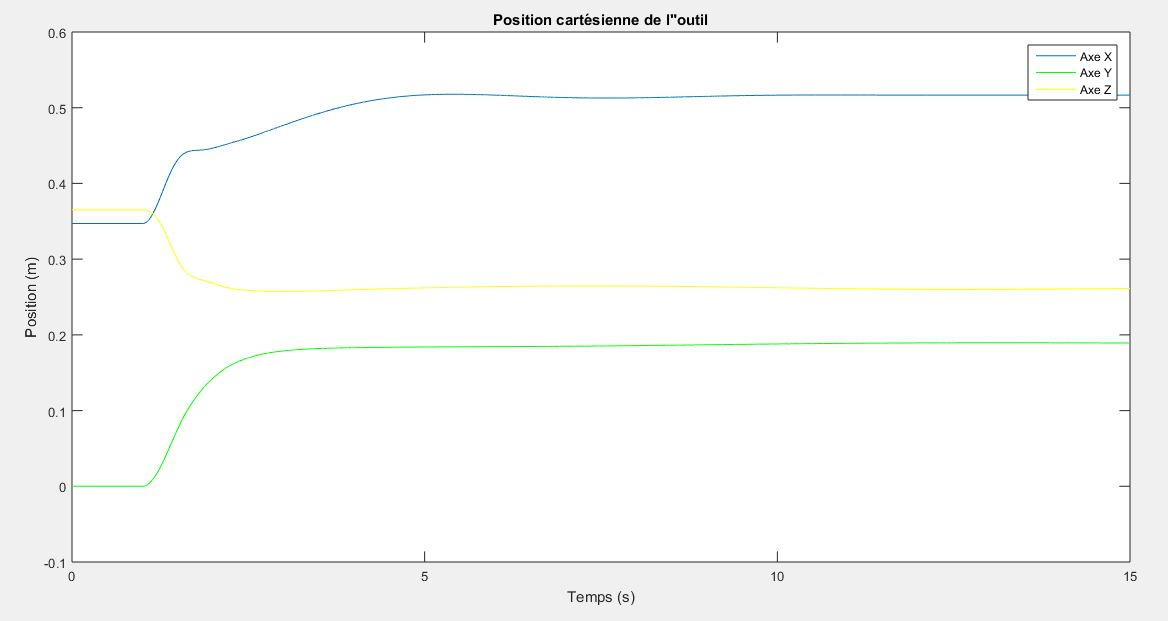
\includegraphics[width=\textwidth]{./PIDtaskxyzgraph.JPG}
		\caption{Réponse temporelle des positions de l'outil à un échelon filtré de consigne pour le système commandé par un PID dans l'espace opérationnel}
		\label{fig:PIDtaskxyzgraph}
	\end{center}
\end{figure}

\begin{figure}[H]
	\begin{center}	
		\captionsetup{justification=centering,margin=1cm}
		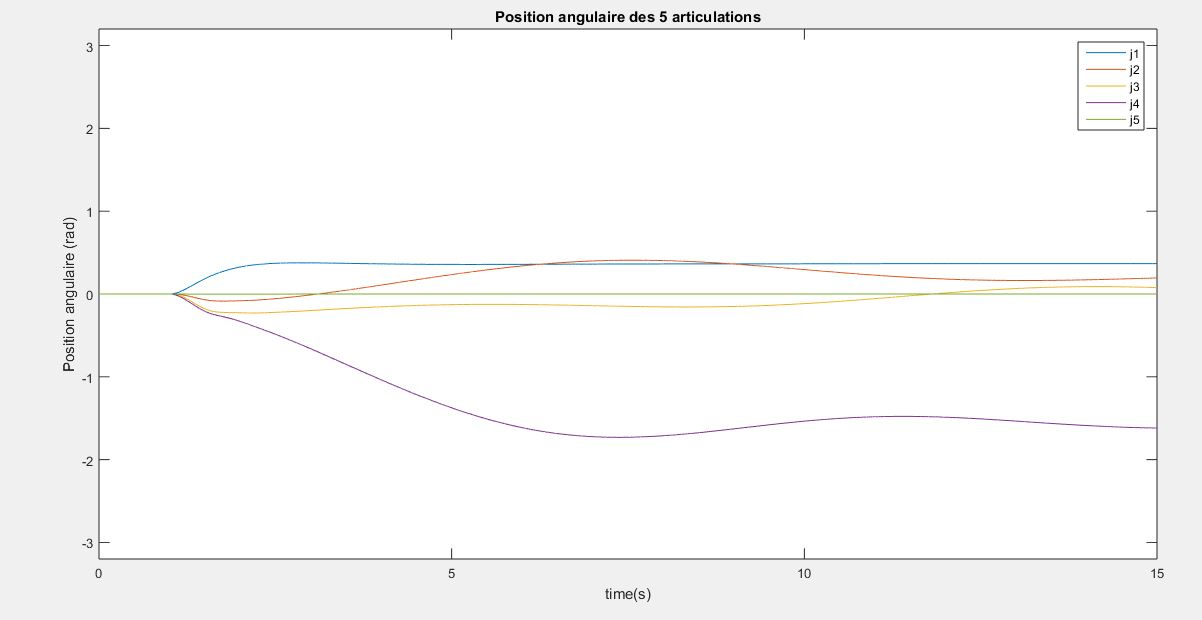
\includegraphics[width=\textwidth]{./PIDtaskartigraph.JPG}
		\caption{Réponse temporelle des positions angulaires des axes du robot à un échelon filtré de consigne pour le système commandé par un PID dans l'espace opérationnel}
		\label{fig:PIDtaskartigraph}
	\end{center}
\end{figure}
\newpage
\begin{figure}[H]
	\begin{center}	
		\captionsetup{justification=centering,margin=1cm}
		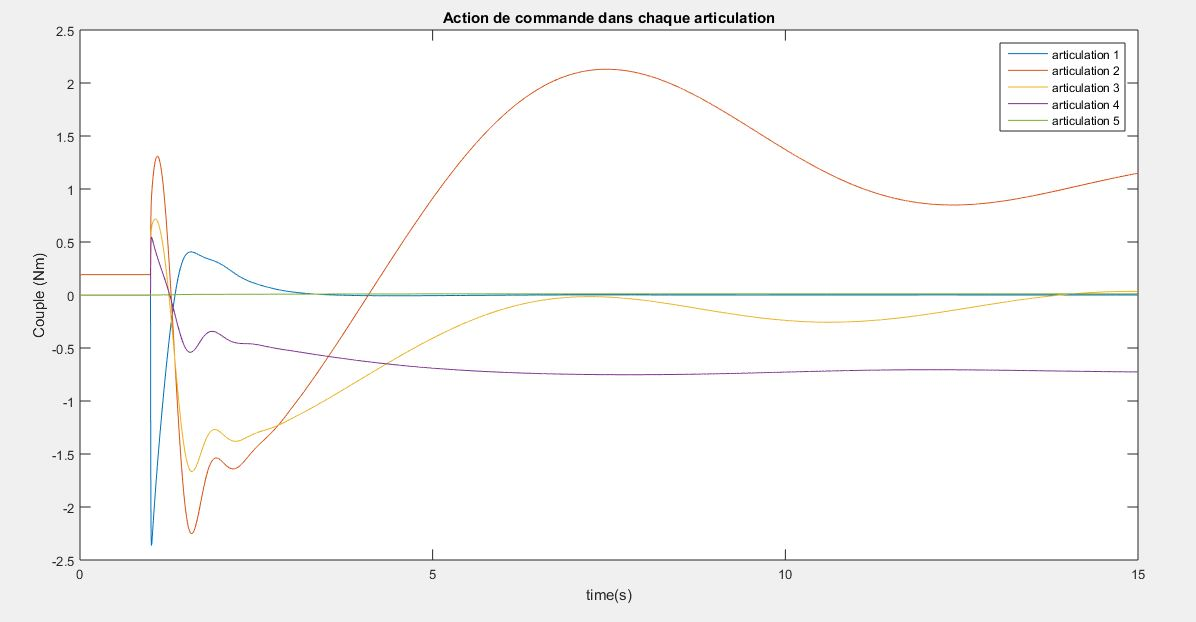
\includegraphics[width=\textwidth]{./PIDtaskcontgraph.JPG}
		\caption{Efforts de commande pour le système commandé par un PID dans l'espace opérationnel}
		\label{fig:PIDtaskcontgraph}
	\end{center}
\end{figure}

